\printbibliography
\newpage

\appendix
\noindent
%\twocolumn
\section{Appendix}
\subsection{A: Segmentation Models}

\begin{figure}[h]
    \begin{tabular}{cc}
    	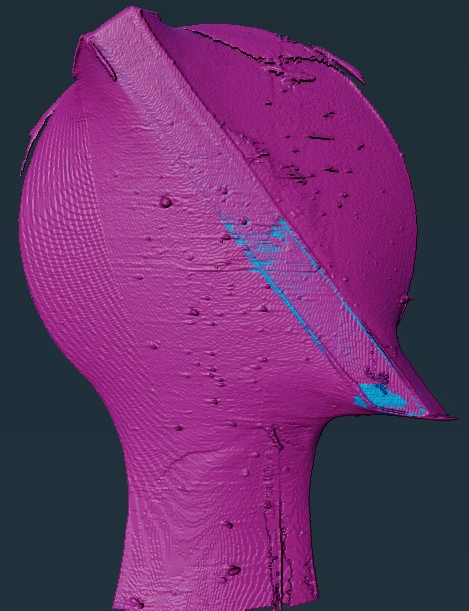
\includegraphics[height=7cm ]{images/avizo_flats/tlys9.jpg} & 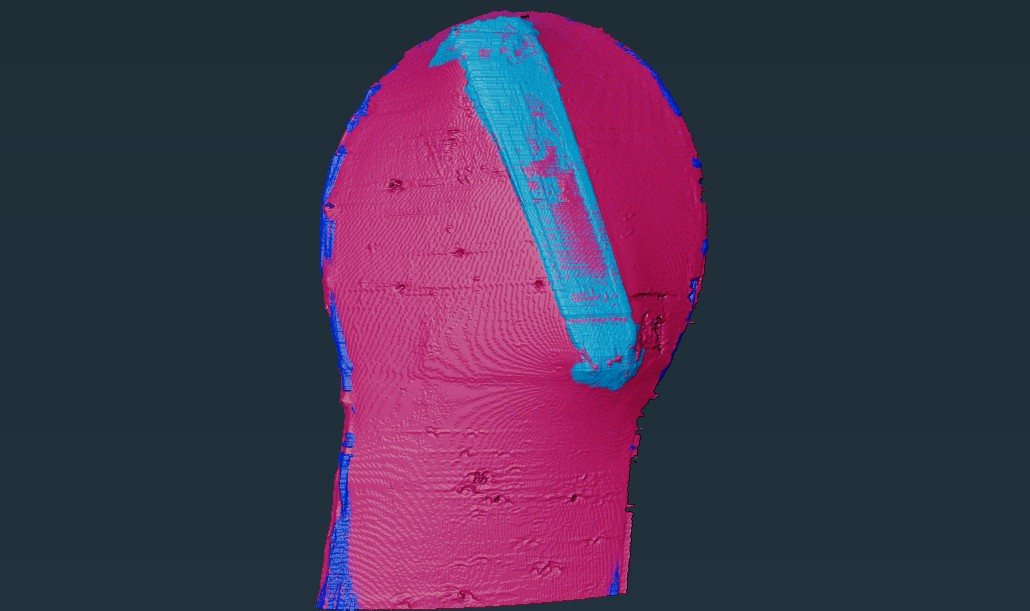
\includegraphics[height=7cm]{images/avizo_flats/tlys2.jpg}
    \end{tabular}
	\caption{Volume rendering in Avizo showing materials of crystal (light blue), liquor (pink), loop (dark blue): Thermolysin 1 (left) and Thermolysin 2 (right)}
 \label{tlys2}
\end{figure}
%\begin{figure}
	%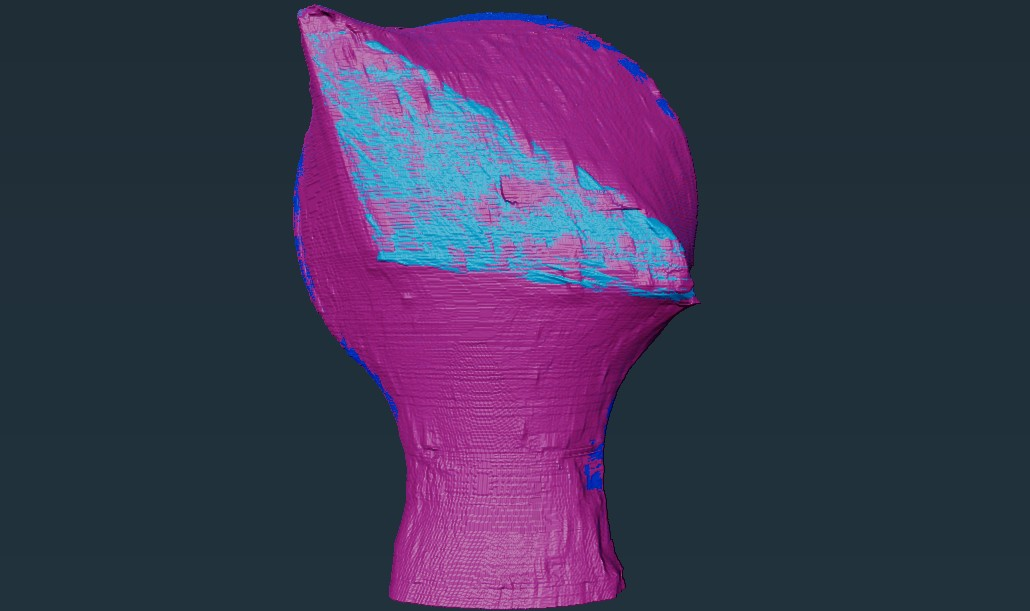
\includegraphics[width=0.5\textwidth]{images/avizo_flats/cas3_1118.jpg}
	%\caption{Volume rendering in Avizo:}
%\label{cas3}
%\end{figure}


\begin{figure}[h]
    \begin{tabular}{cc}
	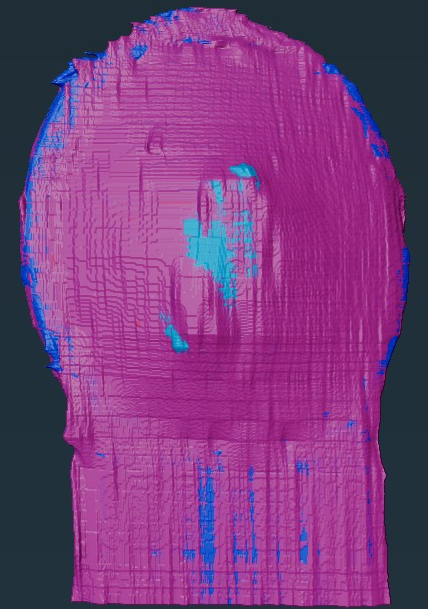
\includegraphics[height=7cm]{images/avizo_flats/ins_con.jpg} & 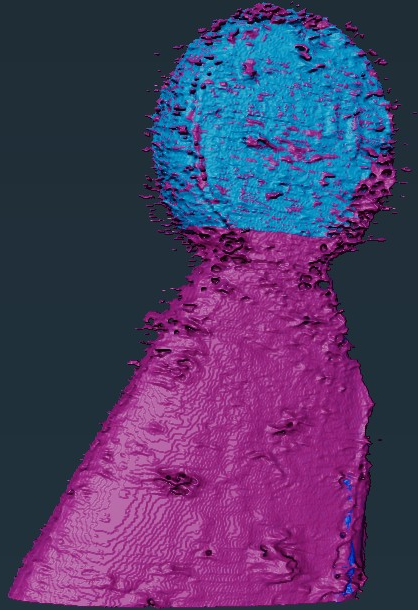
\includegraphics[height=7cm]{images/avizo_flats/ins_ls.jpg}
    \end{tabular}
	\caption{Volume rendering in Avizo showing materials of crystal (light blue), liquor (pink), loop (dark blue): Insulin control crystal (left) and laser-shaped crystal (right)}
 \label{avizo_insulin}
\end{figure}


\begin{figure}
    \begin{tabular}{cc}
	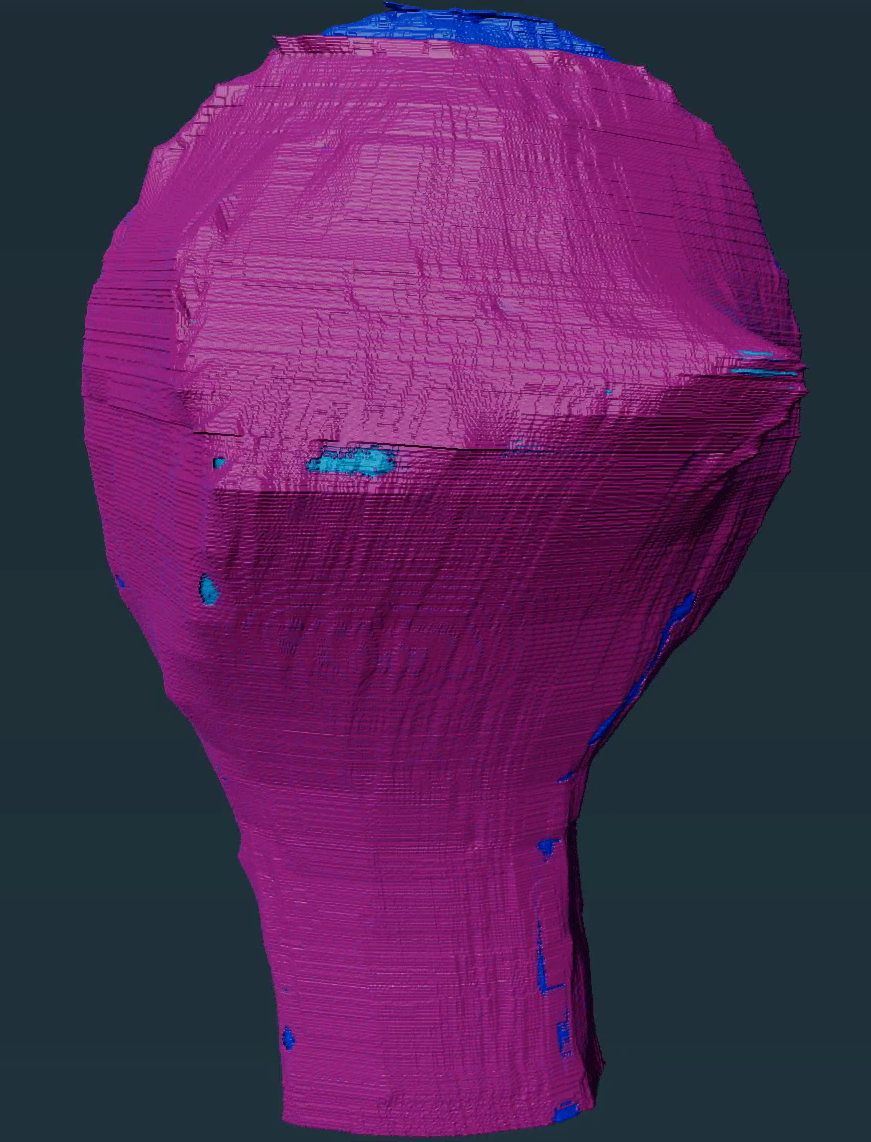
\includegraphics[height=7cm]{images/avizo_flats/prot_con.png} & 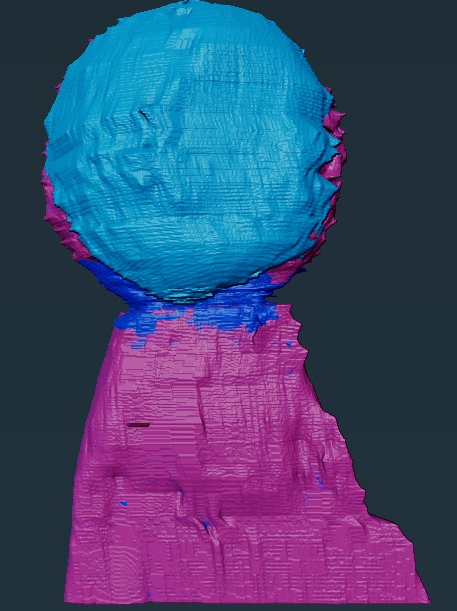
\includegraphics[height=7cm]{images/avizo_flats/prot_ls.jpg}
    \end{tabular}
    \caption{Volume rendering in Avizo showing materials of crystal (light blue), liquor (pink), loop (dark blue): Proteinase-K control crystal (left) and laser-shaped crystal (right)}
    \label{avizo_proteinasek}
\end{figure}


\onecolumn


\newpage
\subsection{B: Plots and Tables}
% Please add the following required packages to your document preamble:
% \usepackage{booktabs}
% \usepackage{multirow}
% \usepackage{graphicx}
\begin{table}[]
\resizebox{\textwidth}{!}{%
\begin{tabular}{@{}lllllll@{}}
\toprule
Crystal                    & Energy               & Processing symmetry group & N.o. datasets      & Transmission       & Kappa & Phi  \\ \midrule
\multirow{23}{*}{Thermolysin 1} & \multirow{7}{*}{3.0} & \multirow{4}{*}{P6122}     & \multirow{4}{*}{4} & \multirow{4}{*}{5}  & -25 & -100 \\
                           &                      &                           &                    &                    & -40   & 70   \\
                           &                      &                           &                    &                    & -35   & -70  \\
                           &                      &                           &                    &                    & 0     & 0    \\
                           &                      & \multirow{3}{*}{P1}       & \multirow{3}{*}{3} & \multirow{3}{*}{5} & -70   & 0    \\
                           &                      &                           &                    &                    & -70   & 120  \\
                           &                      &                           &                    &                    & -70   & -120 \\ \cmidrule(l){2-7} 
                           & \multirow{8}{*}{3.5} & \multirow{5}{*}{P6122}    & \multirow{5}{*}{5} & \multirow{5}{*}{1} & 0     & 0    \\
                           &                      &                           &                    &                    & -15   & 100  \\
                           &                      &                           &                    &                    & -25   & -100 \\
                           &                      &                           &                    &                    & -40   & 70   \\
                           &                      &                           &                    &                    & -35   & -70  \\
                           &                      & \multirow{3}{*}{P1}       & \multirow{3}{*}{3} & \multirow{3}{*}{1} & -70   & -120 \\
                           &                      &                           &                    &                    & -70   & 0    \\
                           &                      &                           &                    &                    & -70   & 120  \\ \cmidrule(l){2-7} 
                           & \multirow{8}{*}{3.8} & \multirow{5}{*}{P6122}    & \multirow{5}{*}{5} & \multirow{5}{*}{1} & 0     & 0    \\
                           &                      &                           &                    &                    & -15   & 100  \\
                           &                      &                           &                    &                    & -25   & -100 \\
                           &                      &                           &                    &                    & -40   & 70   \\
                           &                      &                           &                    &                    & -35   & -70  \\ \cmidrule(l){3-7} 
                           &                      & \multirow{3}{*}{P1}       & \multirow{3}{*}{3} & \multirow{3}{*}{1} & -70   & -120 \\
                           &                      &                           &                    &                    & -70   & 0    \\
                           &                      &                           &                    &                    & -70   & 120  \\ \midrule
\multirow{9}{*}{Thermolysin 2}  & \multirow{4}{*}{3.0} & \multirow{4}{*}{P6122, P1} & \multirow{4}{*}{4} & \multirow{4}{*}{20} & 0   & 0    \\
                           &                      &                           &                    &                    & -70   & -100 \\
                           &                      &                           &                    &                    & -70   & 0    \\
                           &                      &                           &                    &                    & -70   & 100  \\ \cmidrule(l){2-7} 
                                & \multirow{5}{*}{3.5} & \multirow{5}{*}{P6122, P1} & \multirow{5}{*}{5} & \multirow{5}{*}{15} & 0   & 0    \\
                           &                      &                           &                    &                    & -70   & -100 \\
                           &                      &                           &                    &                    & -70   & 0    \\
                           &                      &                           &                    &                    & -70   & 100  \\
                           &                      &                           &                    &                    & 0     & 0    \\ \midrule
Insulin 1                  & 3.0                  & I213                      & 1                  & 20                 & 0     & 0    \\ \midrule
Insulin 2                  & 3.0                  & I213                      & 1                  & 15                 & 0     & 0    \\ \midrule
Proteinase-K 1             & 3.0                  & P43212                    & 1                  & 20                 & 0     & 0    \\ \midrule
Proteinase-K 2             & 3.0                  & P43212                    & 1                  & 20                 & 0     & 0    \\ \midrule
\multirow{4}{*}{Thaumatin} & 3.0                  & \multirow{4}{*}{P41212}   & 1                  &                    & 0     & 0    \\
                           & 3.5                  &                           & 1                  &                    & 0     & 0    \\
                           & 4.0                  &                           & 1                  &                    & 0     & 0    \\
                           & 4.5                  &                           & 1                  &                    & 0     & 0    \\ \bottomrule
\end{tabular}%
}
\caption{Diffraction Data Collection Parameters; collected at beamline I23, Diamond Light Source, UK.}
\label{diffration_table}
\end{table}

%\caption{Diffraction Data Collection Parameters}







% Please add the following required packages to your document preamble:
% \usepackage{booktabs}
% \usepackage{multirow}
% \usepackage{graphicx}
% \usepackage[table,xcdraw]{xcolor}
% Beamer presentation requires \usepackage{colortbl} instead of \usepackage[table,xcdraw]{xcolor}
\begin{table}[h]
\resizebox{\textwidth}{!}{%
\begin{tabular}{@{}lllll@{}}
\toprule
Crystal                          & Energy & N.o. datasets & Exposure time (s per 0.2 deg) & Notes                          \\ \midrule
                                 & 3.0    & 4             & 0.35                          &                                \\
                                 & 3.5    & 5             & 0.25                          &                                \\
\multirow{-3}{*}{Thermolysin 1}  & 3.8    & 5             & 0.22                          &                                \\
                                 & 3.0    & 4             & 0.25                          &                                \\
\multirow{-2}{*}{Thermolysin 2}  & 3.5    & 5             & 0.3                           &                                \\
                                 & 3.0    & 1             & 0.3                           &                                \\
\multirow{-2}{*}{Insulin 1}      & 3.5    & 1             & 0.25                          & \multirow{-2}{*}{laser-shaped} \\
                                 & 3.0    & 1             & 0.3                           &                                \\
\multirow{-2}{*}{Insulin 2}      & 3.5    & 1             & 0.25                          & \multirow{-2}{*}{control}      \\
                                 & 3.0    & 1             & 0.3                           &                                \\
\multirow{-2}{*}{Proteinase-K 1} & 3.5    & 1             & 0.25                          & \multirow{-2}{*}{laser-shaped} \\
                                 & 3.0    & 1             & 0.3                           &                                \\
\multirow{-2}{*}{Proteinase-K 2} & 3.5    & 1             & 0.25                          & \multirow{-2}{*}{control}      \\
                                 & 2.4    & 2             & 0.35                          &                                \\
                                 & 3.0    & 2             & 0.3                           &                                \\
\multirow{-3}{*}{Lysozyme}       & 3.5    & 3             & 0.2                           &                                \\
                                 & 3.0    & 1             & 0.35                          &                                \\
                                 & 3.5    & 1             & 0.2                           &                                \\
                                 & 4.0    & 1             & 0.28                          &                                \\
\multirow{-4}{*}{Thaumatin}      & 4.5    & 1             & 0.18                          &       \\
\bottomrule
\end{tabular}%
}

\caption{Tomography Data Collection Parameters; collected using the goniometer at $\kappa$, $\phi$ = 0$\deg$, 0$\deg$ at the I23 endstation, Diamond Light Source, UK.}
\label{tomo_table}
\end{table}




% Please add the following required packages to your document preamble:
% \usepackage{booktabs}
% \usepackage{graphicx}
\begin{table}[h]
\resizebox{\textwidth}{!}{%
\begin{tabular}{@{}lllll@{}}
\toprule
Energy (eV) & Attenuation length (µm) & Theoretical coefficient (1/µm) & Experimental coefficient (1/µm) & Percentage Difference (\%) \\ \midrule
3000 & 60.3724 & 0.016564 & 0.01615  & -2.4973  \\
3500 & 95.0695 & 0.010519 & 0.010281 & -2.25611 \\
4000 & 141.783 & 0.007053 & 0.00696  & -1.32401 \\
4500 & 202.56  & 0.004937 & 0.00491  & -0.53778 \\
5000 & 279.179 & 0.003582 & 0.003625 & 1.215159 \\
6000 & 488.075 & 0.002049 & 0.002179 & 6.345384 \\ \bottomrule
\end{tabular}%
}
\caption{Experimentally calculated santovac absorption coefficients from AnACor at 50 \% material acceptance. Attenuation length calculated based on chemical formula \ce{C30H22O4} and density 1.195 \unit{\gram\per\cubic\cm} on the Center for X-Ray Optics \href{https://henke.lbl.gov/optical_constants/atten2.html}{X-ray Attenuation Length} platform.}
\label{santovac_table}
\end{table}


% Please add the following required packages to your document preamble:
% \usepackage{booktabs}
% \usepackage{graphicx}
\begin{table}[h]
\resizebox{\textwidth}{!}{%
\begin{tabular}{@{}lllll@{}}
\toprule
Energy (eV) & Attenuation length (µm) & Theoretical coefficient (1/µm) & Experimental coefficient (1/µm) & Percentage Difference (\%) \\ \midrule
3000 & 60.3724 & 0.016564 & 0.01615  & -2.4973  \\
3500 & 95.0695 & 0.010519 & 0.010281 & -2.25611 \\
4000 & 141.783 & 0.007053 & 0.00696  & -1.32401 \\
4500 & 202.56  & 0.004937 & 0.00491  & -0.53778 \\
5000 & 279.179 & 0.003582 & 0.003625 & 1.215159 \\
6000 & 488.075 & 0.002049 & 0.002179 & 6.345384 \\ \bottomrule
\end{tabular}%
}
\caption{Experimentally calculated ethylene glycol absorption coefficients from AnACor at 50 \% material acceptance. Attenuation length calculated based on chemical formula \ce{C2H6O2} and density 1.195 \unit{\gram\per\cubic\cm} on the Center for X-Ray Optics \href{https://henke.lbl.gov/optical_constants/atten2.html}{X-ray Attenuation Length} platform.}
\label{ethylene_table}
\end{table}



% Please add the following required packages to your document preamble:
% \usepackage{booktabs}
% \usepackage{multirow}
% \usepackage{graphicx}
% Please add the following required packages to your document preamble:
% \usepackage{booktabs}
% \usepackage{multirow}
% \usepackage{graphicx}
\begin{table}[h]
\resizebox{\textwidth}{!}{%
\begin{tabular}{@{}llllll@{}}
\toprule
\multirow{3}{*}{Atom, Energy} &
  \multirow{3}{*}{\begin{tabular}[c]{@{}l@{}}Theoretical f'\\ (used in Phenix.refine)\end{tabular}} &
  \multirow{3}{*}{Theoretical f"} &
  \multicolumn{3}{c}{Experimental f"} \\
                             &                            &                           & \multicolumn{1}{c}{AC} & \multicolumn{1}{c}{SH} & \multicolumn{1}{c}{ACSH} \\ \cmidrule(l){4-6} 
                             &                            &                           & \multicolumn{3}{c}{\% Difference}                                          \\ \midrule
\multirow{2}{*}{S, 3 \unit{keV}}    & \multirow{2}{*}{-0.75226}  & \multirow{2}{*}{3.059391} & 2.49912                & 2.45008                & 3.03552                  \\
                             &                            &                           & -18.3132               & -19.9161               & -0.78025                 \\ \midrule
\multirow{2}{*}{ZN, 3.0 \unit{keV}} & \multirow{2}{*}{3.56E-02}  & \multirow{2}{*}{3.764636} & 2.83766                & 2.36456                & 2.68316                  \\
                             &                            &                           & -24.6233               & -37.1902               & -28.7272                 \\ \midrule
\multirow{2}{*}{S, 3.5 \unit{keV}}  & \multirow{2}{*}{-8.16E-02} & \multirow{2}{*}{2.390438} & 2.21949                & 2.24339                & 2.42956                  \\
                             &                            &                           & -7.15133               & -6.15151               & 1.636604                 \\ \midrule
\multirow{2}{*}{ZN, 3.5 \unit{keV}}  & \multirow{2}{*}{-6.15E-02} & \multirow{2}{*}{2.912471} & 2.36736                & 2.1546                 & 2.62166                  \\
                             &                            &                           & -18.7164               & -26.0216               & -9.98503                 \\ \bottomrule
\end{tabular}%
}

\caption{Phenix Refinement on Thermolysin 2 reflection data, for sulphur and zinc at 3.0, 3.5 \unit{keV}.}
\label{phenix_table}
\end{table}



\begin{figure}[h]
    \centering
    \begin{tabular}{cc}
    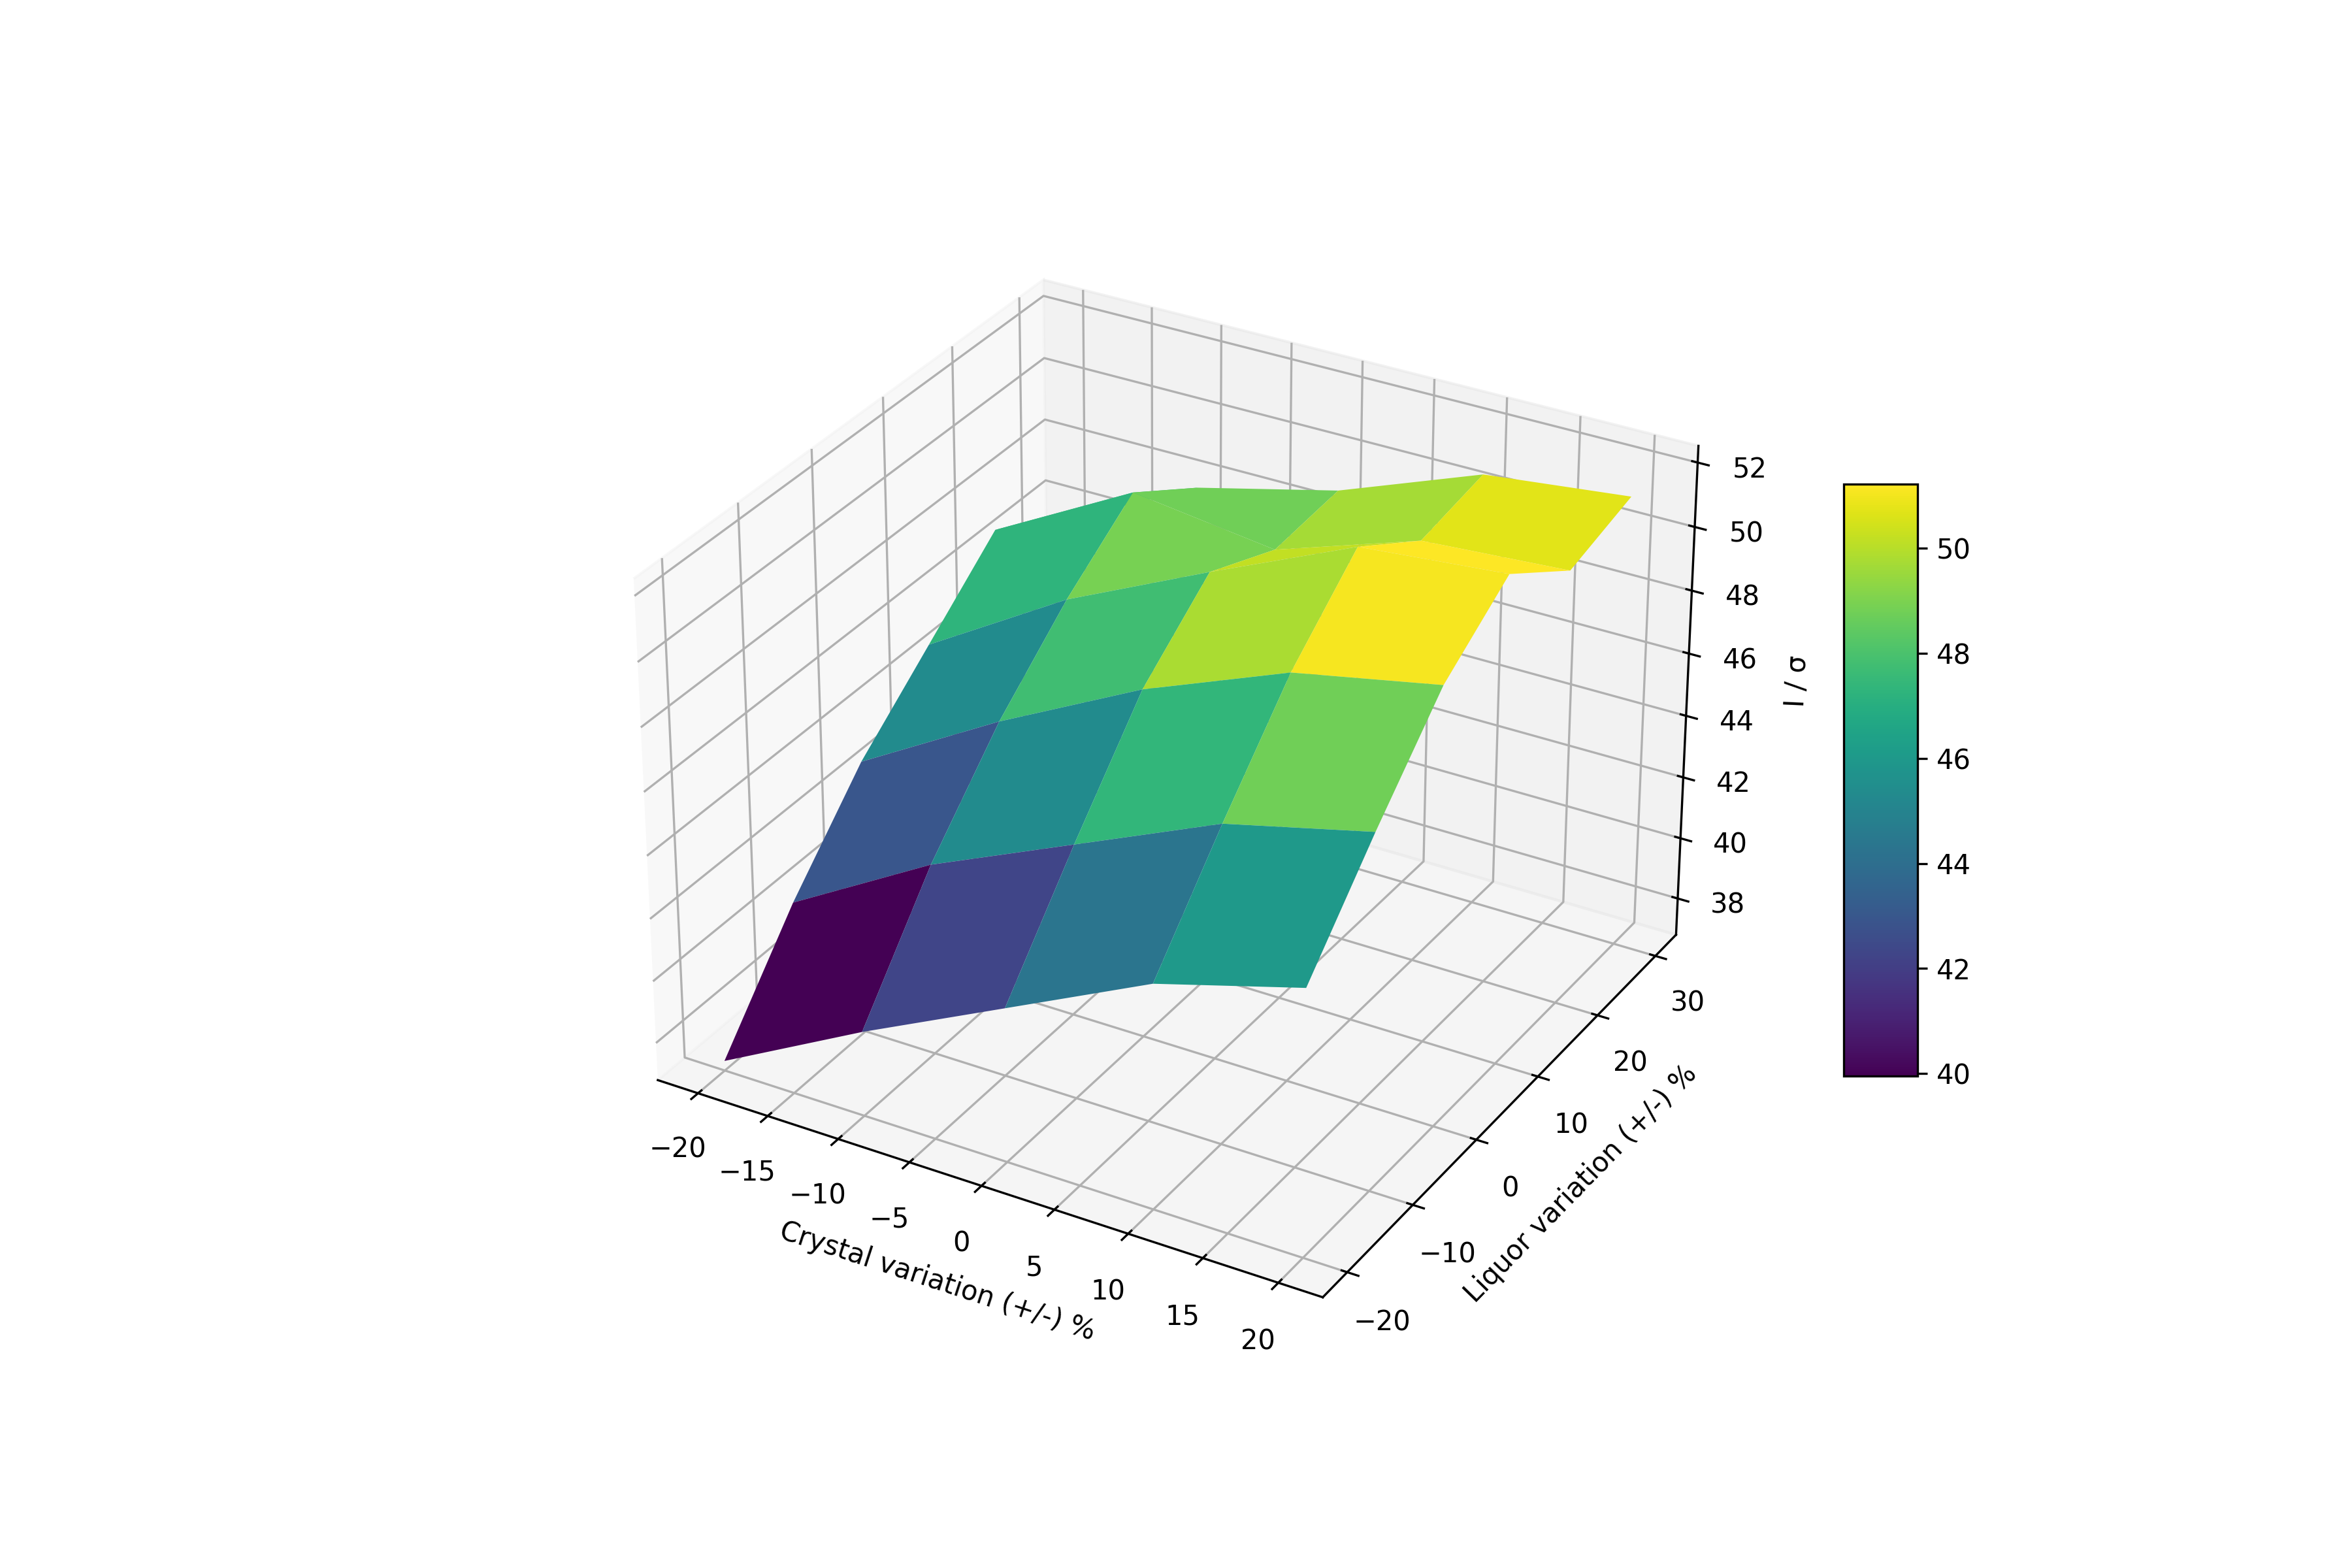
\includegraphics[width = 0.5\textwidth]{plots/exp0/cld_merged_Isig.png} & 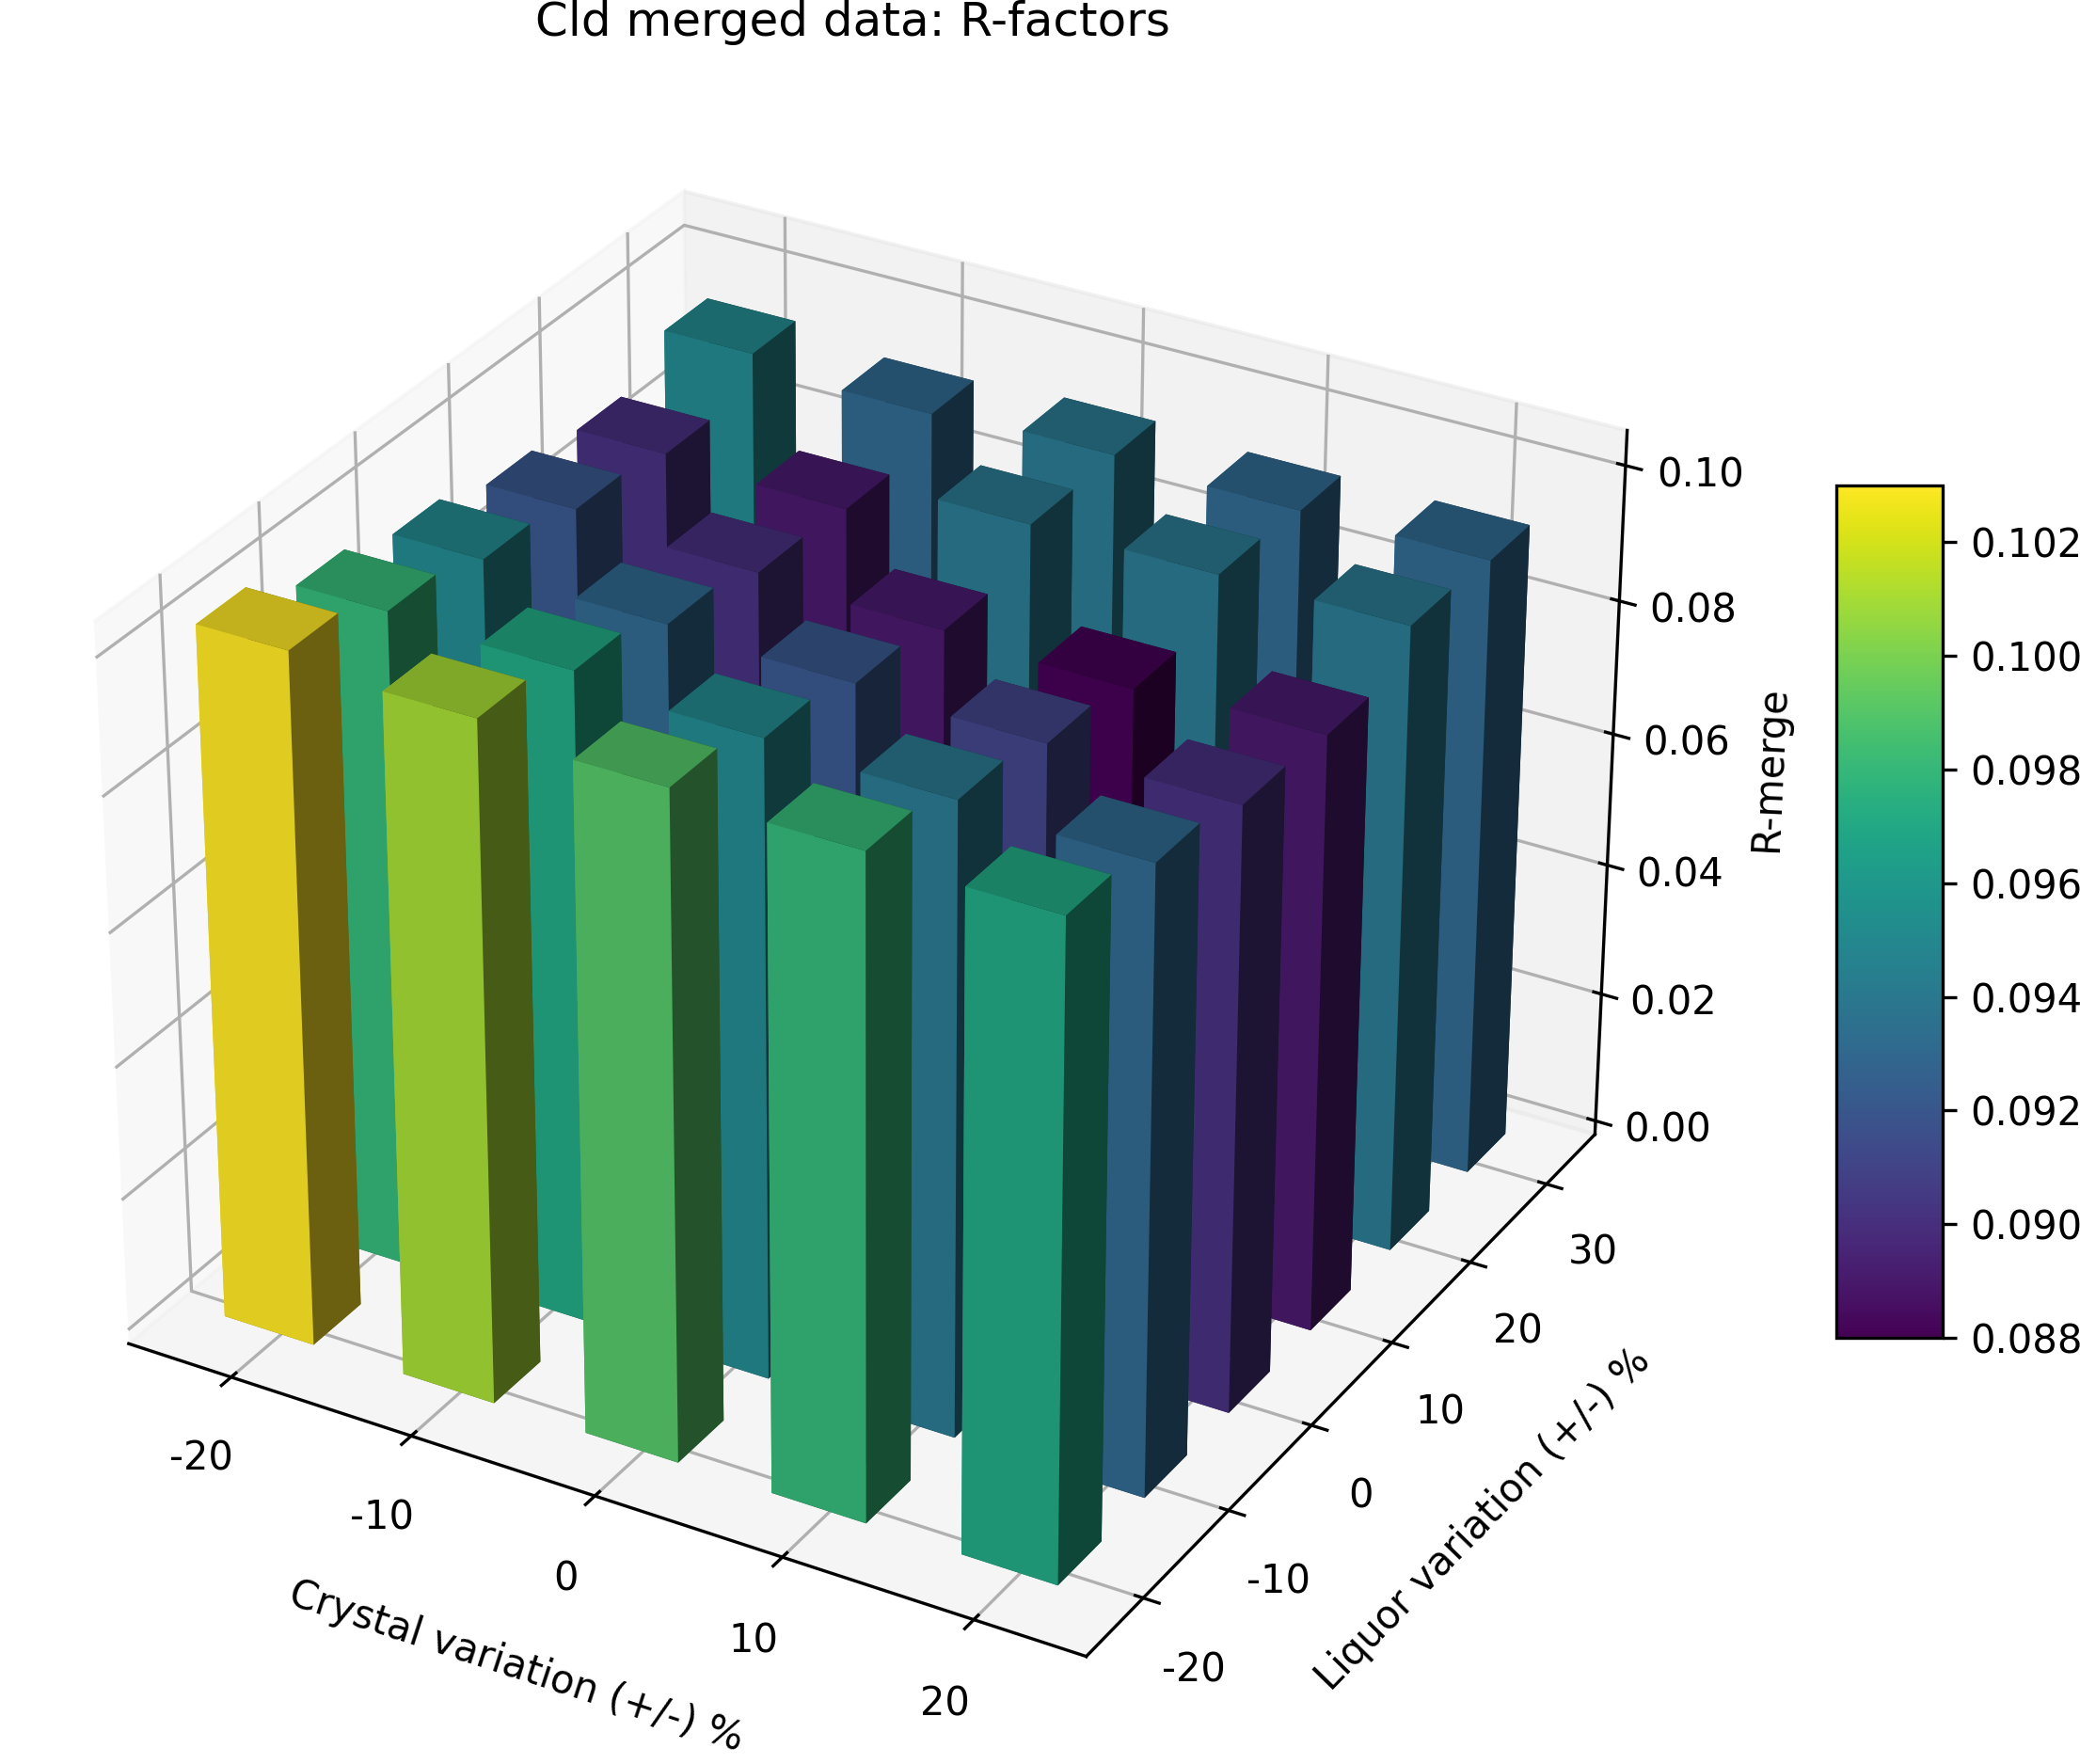
\includegraphics[trim={7.1cm 1cm 4.3cm 1cm},clip,width = 0.5\textwidth]{plots/exp0/cld_merged_rmerge.png} %[trim={5cm 0 5cm 0},clip]
    \end{tabular}
    \caption{Effects of varying the experimental Cld crystal and liquor absorption coefficients in Lu \textit{et al.} calculated by AnACor.}
    \label{fig:cld_stats}
\end{figure}

\begin{figure}[H]
    \centering
    \begin{tabular}{cc}
    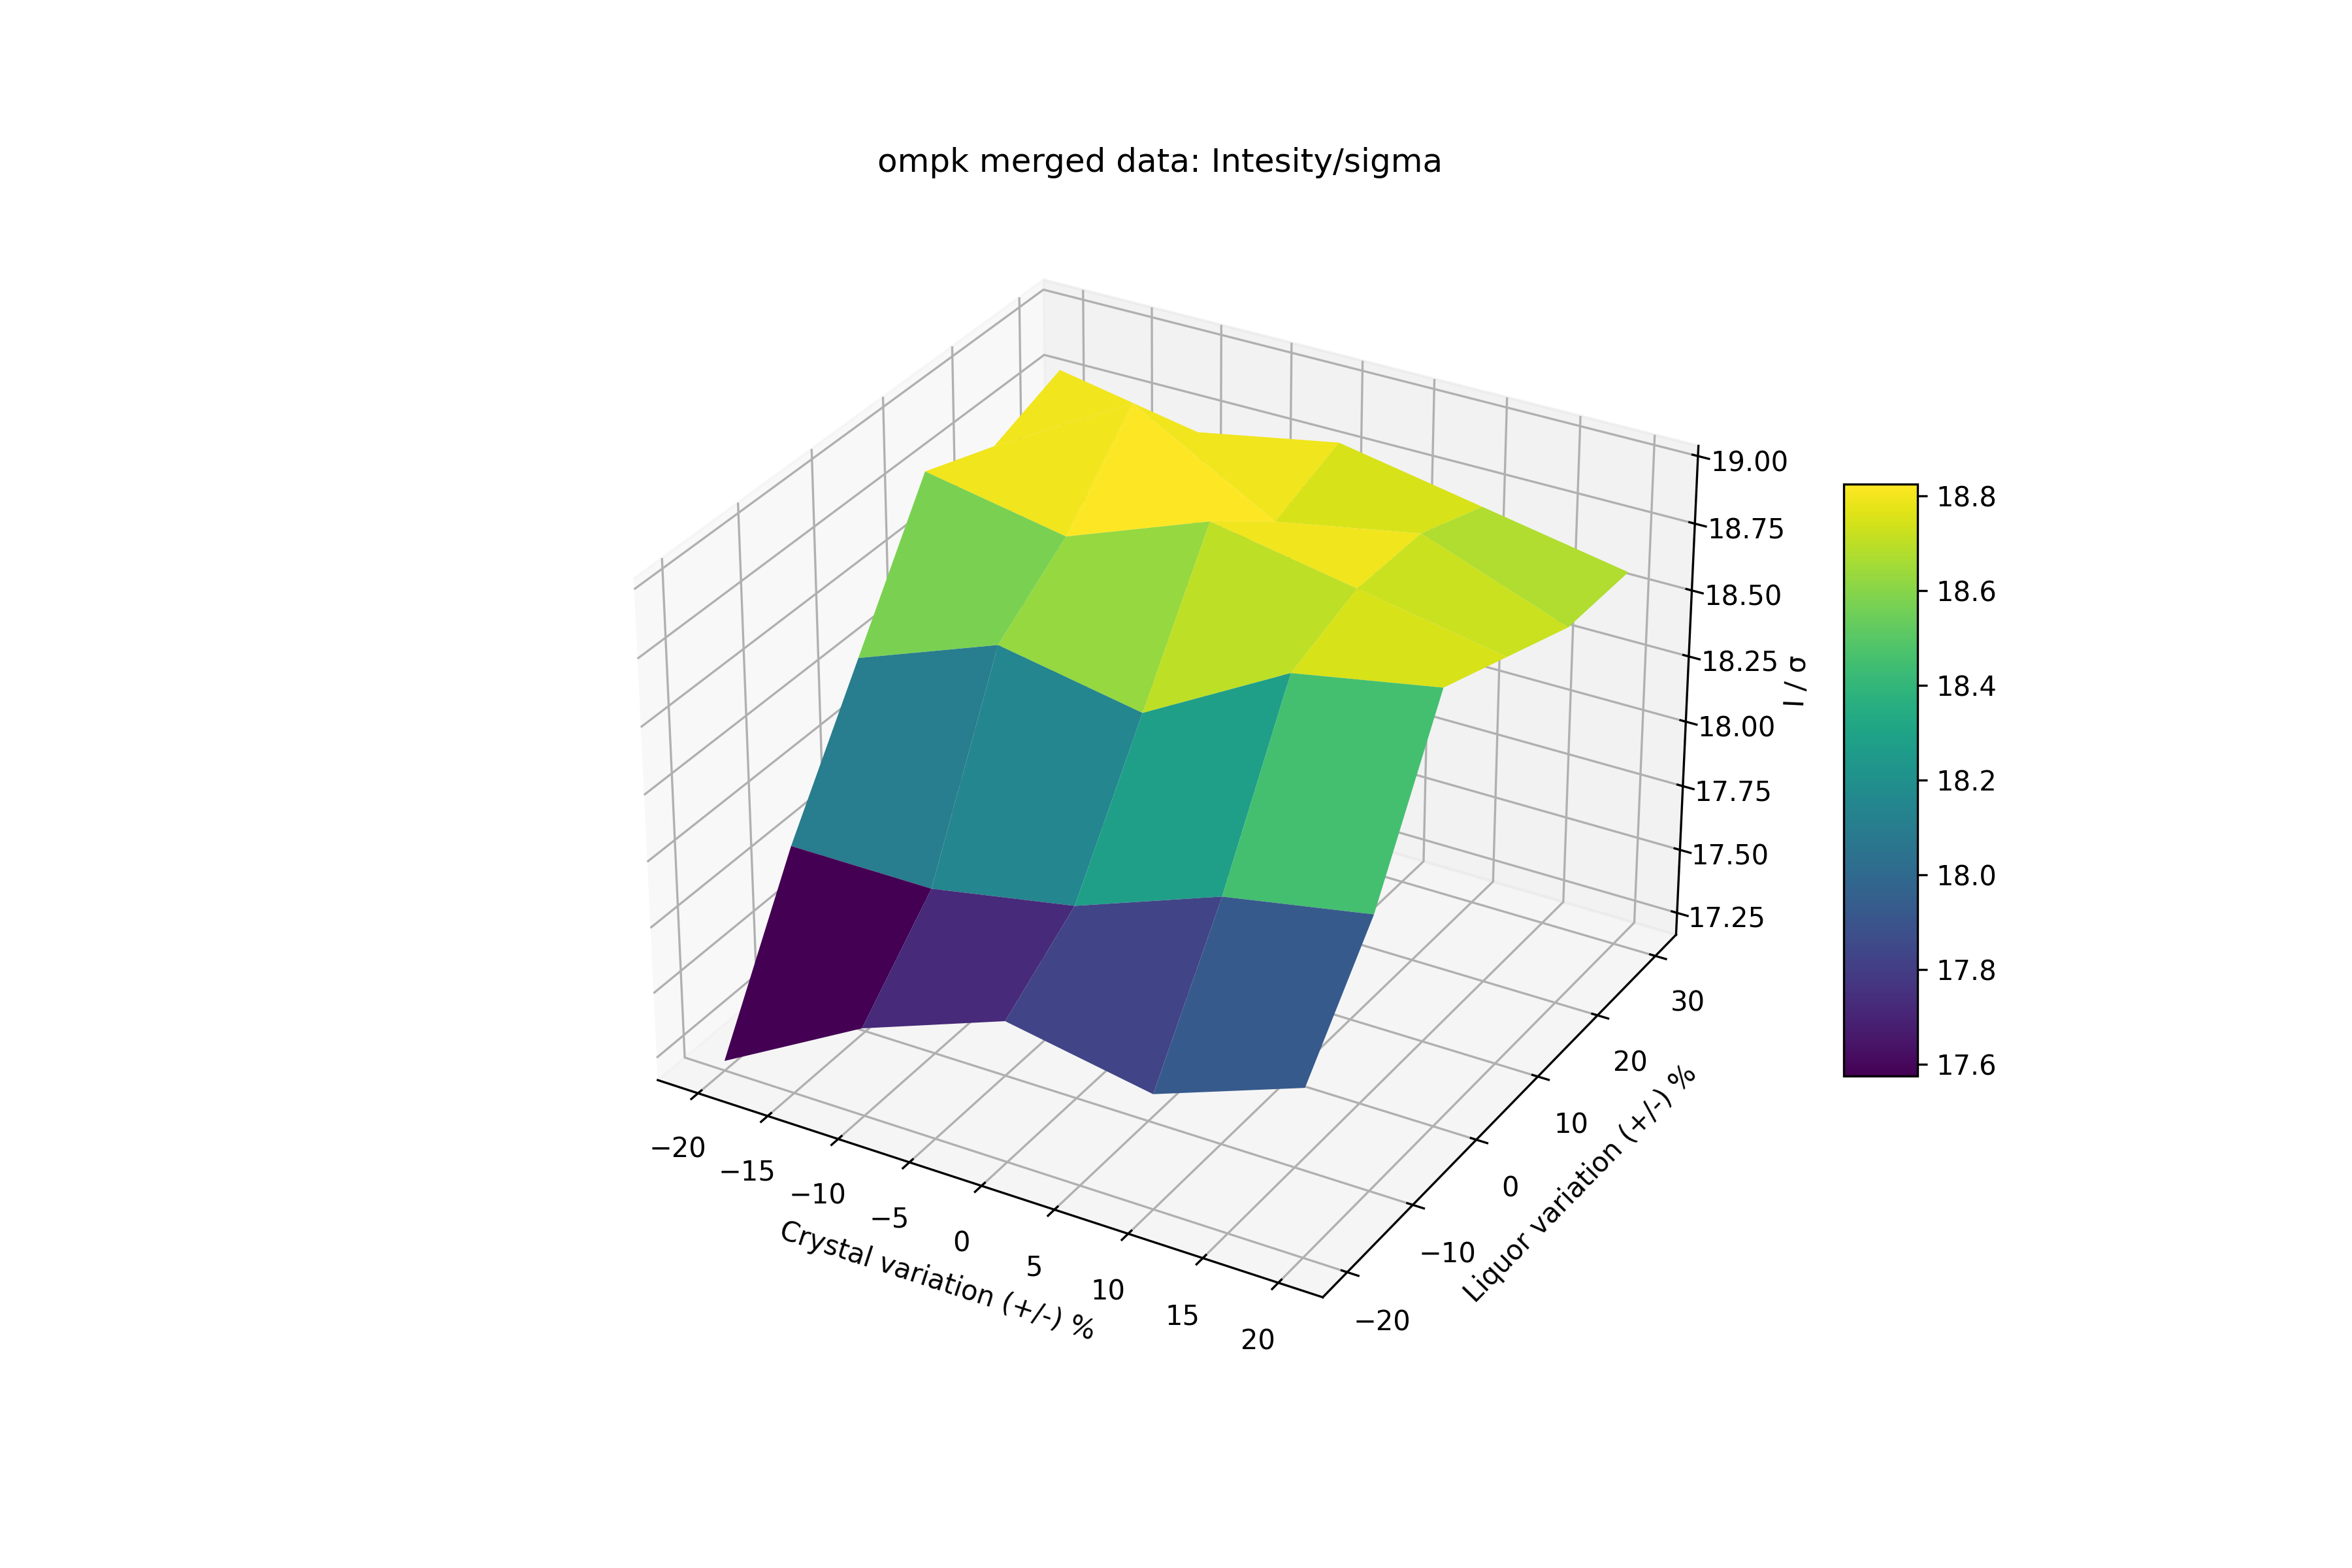
\includegraphics[width = 0.5\textwidth]{plots/exp0/ompk_merged_Isig.png} & 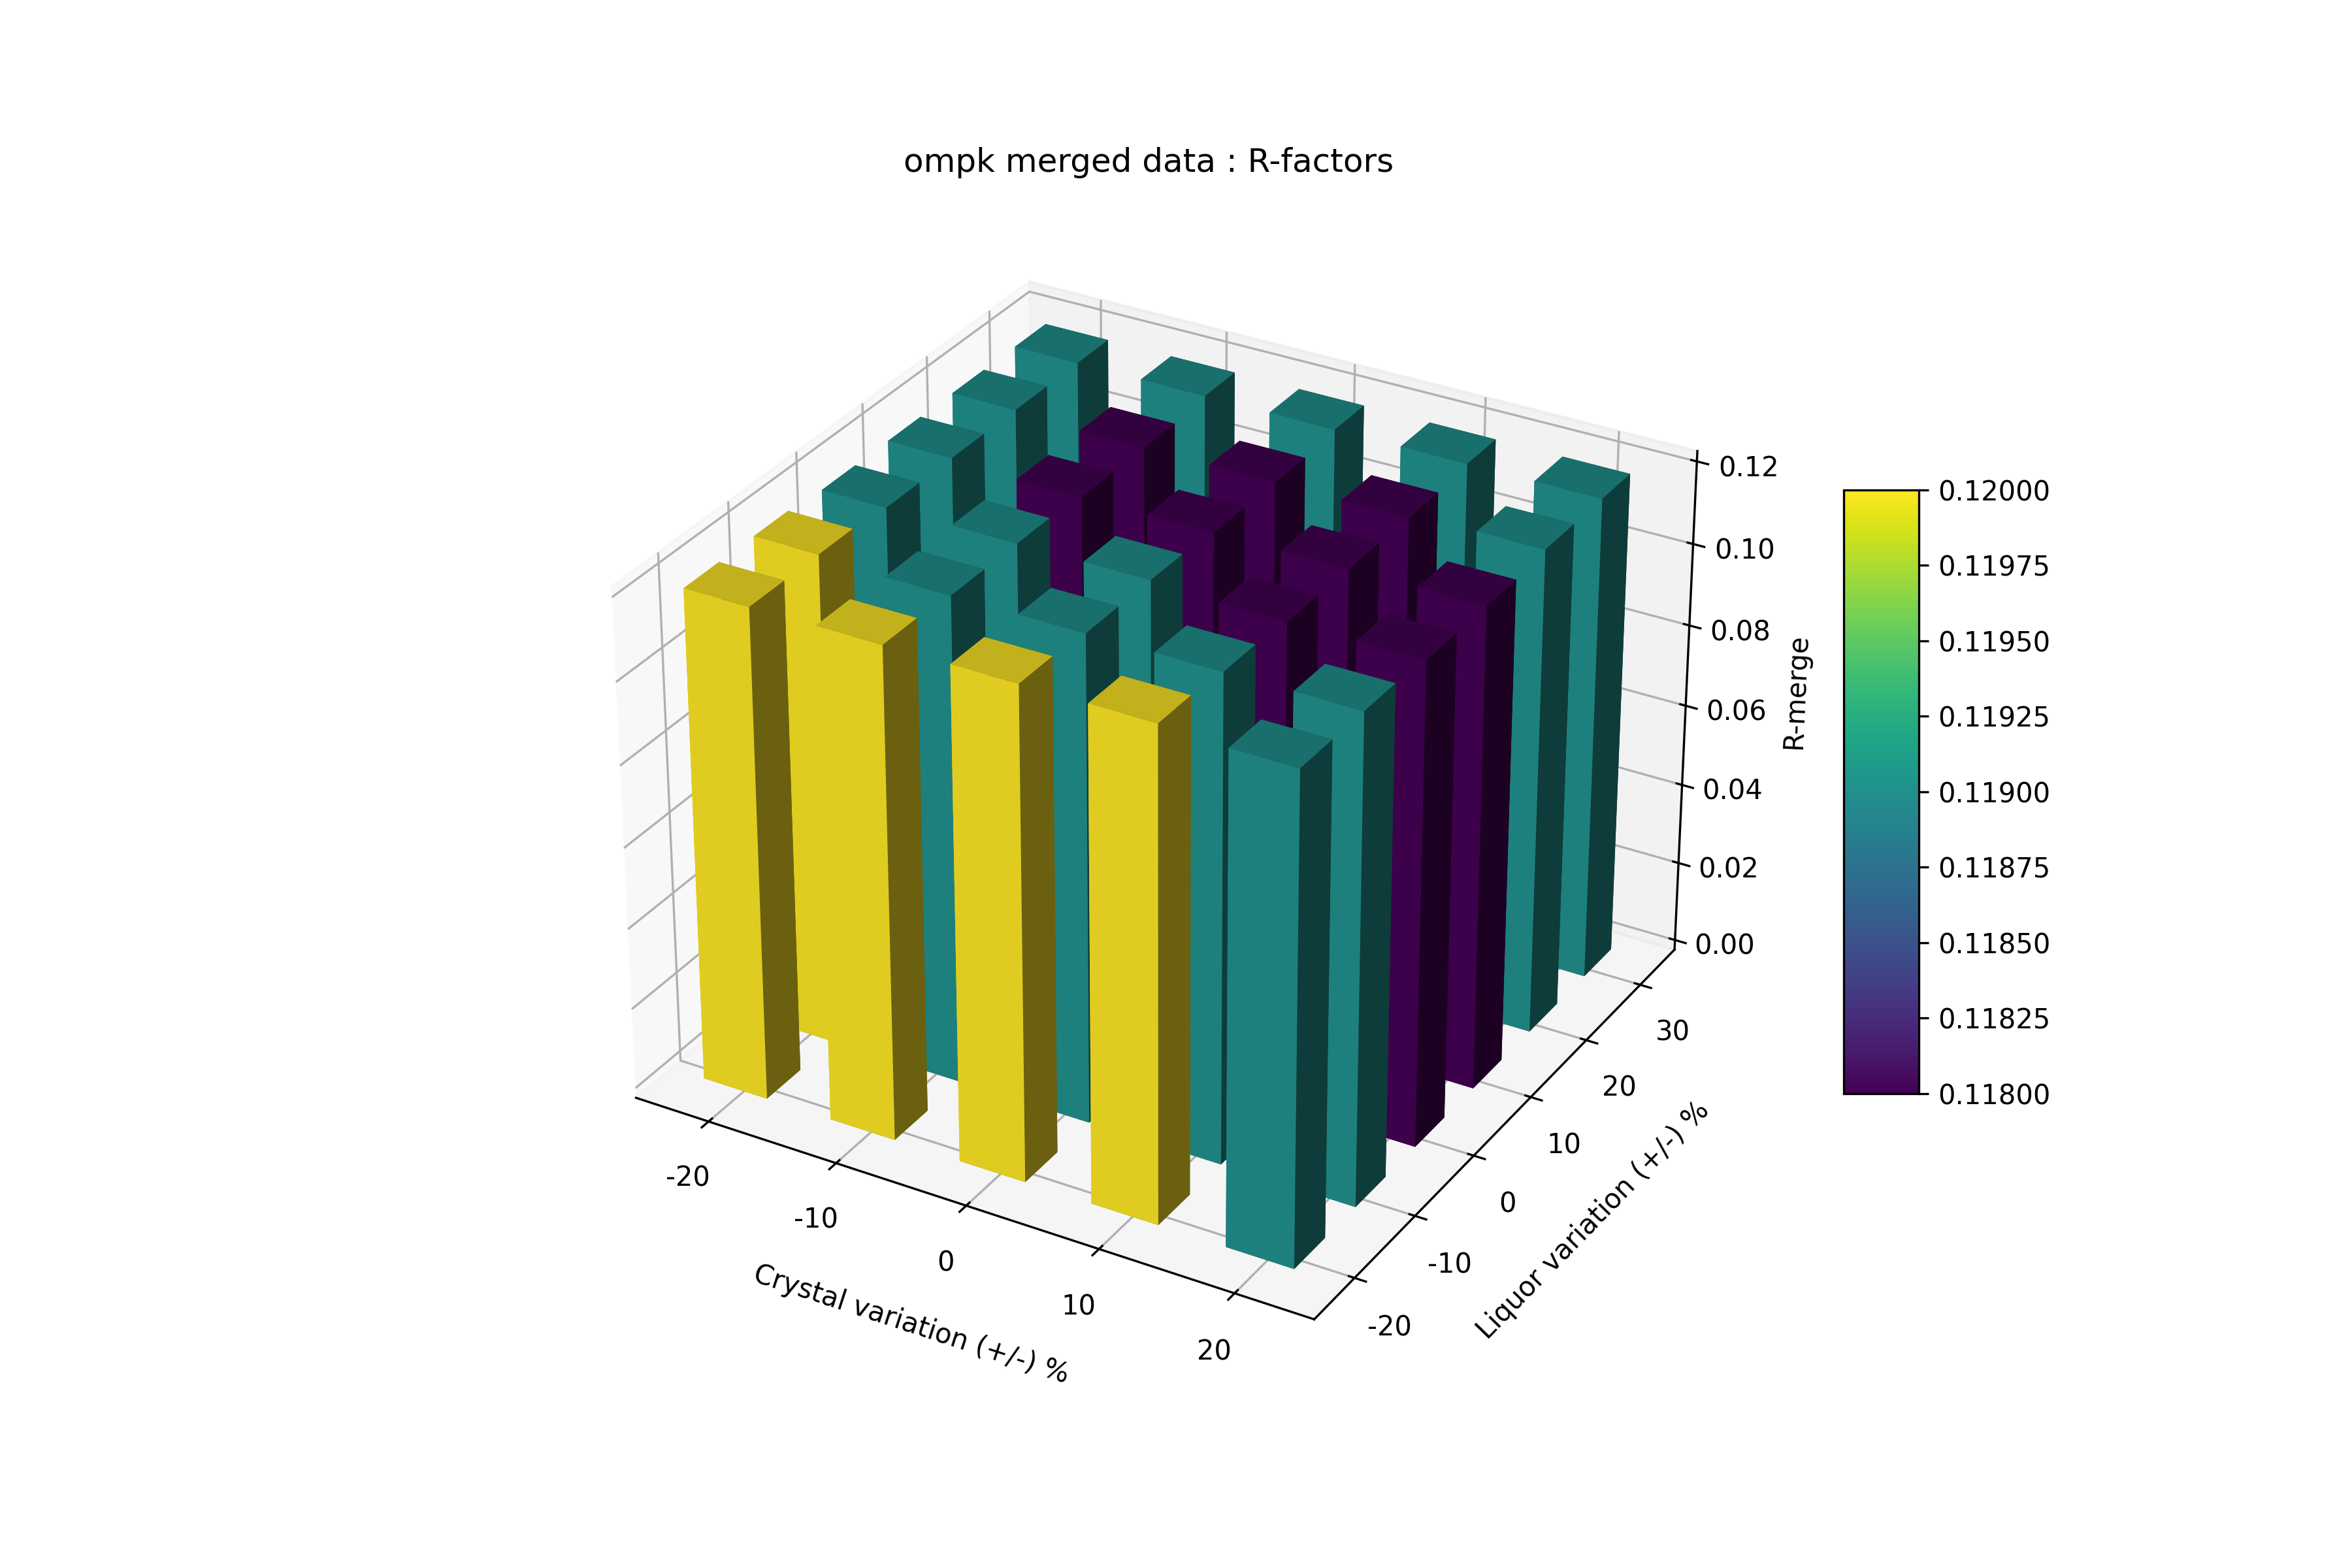
\includegraphics[width = 0.5\textwidth]{plots/exp0/ompk_merged_rmerge.png}
    \end{tabular}
    \caption{Effects of varying the experimental Ompk crystal and liquor absorption coefficients in Lu \textit{et al.} calculated by AnACor.}
    \label{fig:ompk_stats}
\end{figure}



\begin{figure}[h]
    \centering
    \begin{tabular}{cc}
    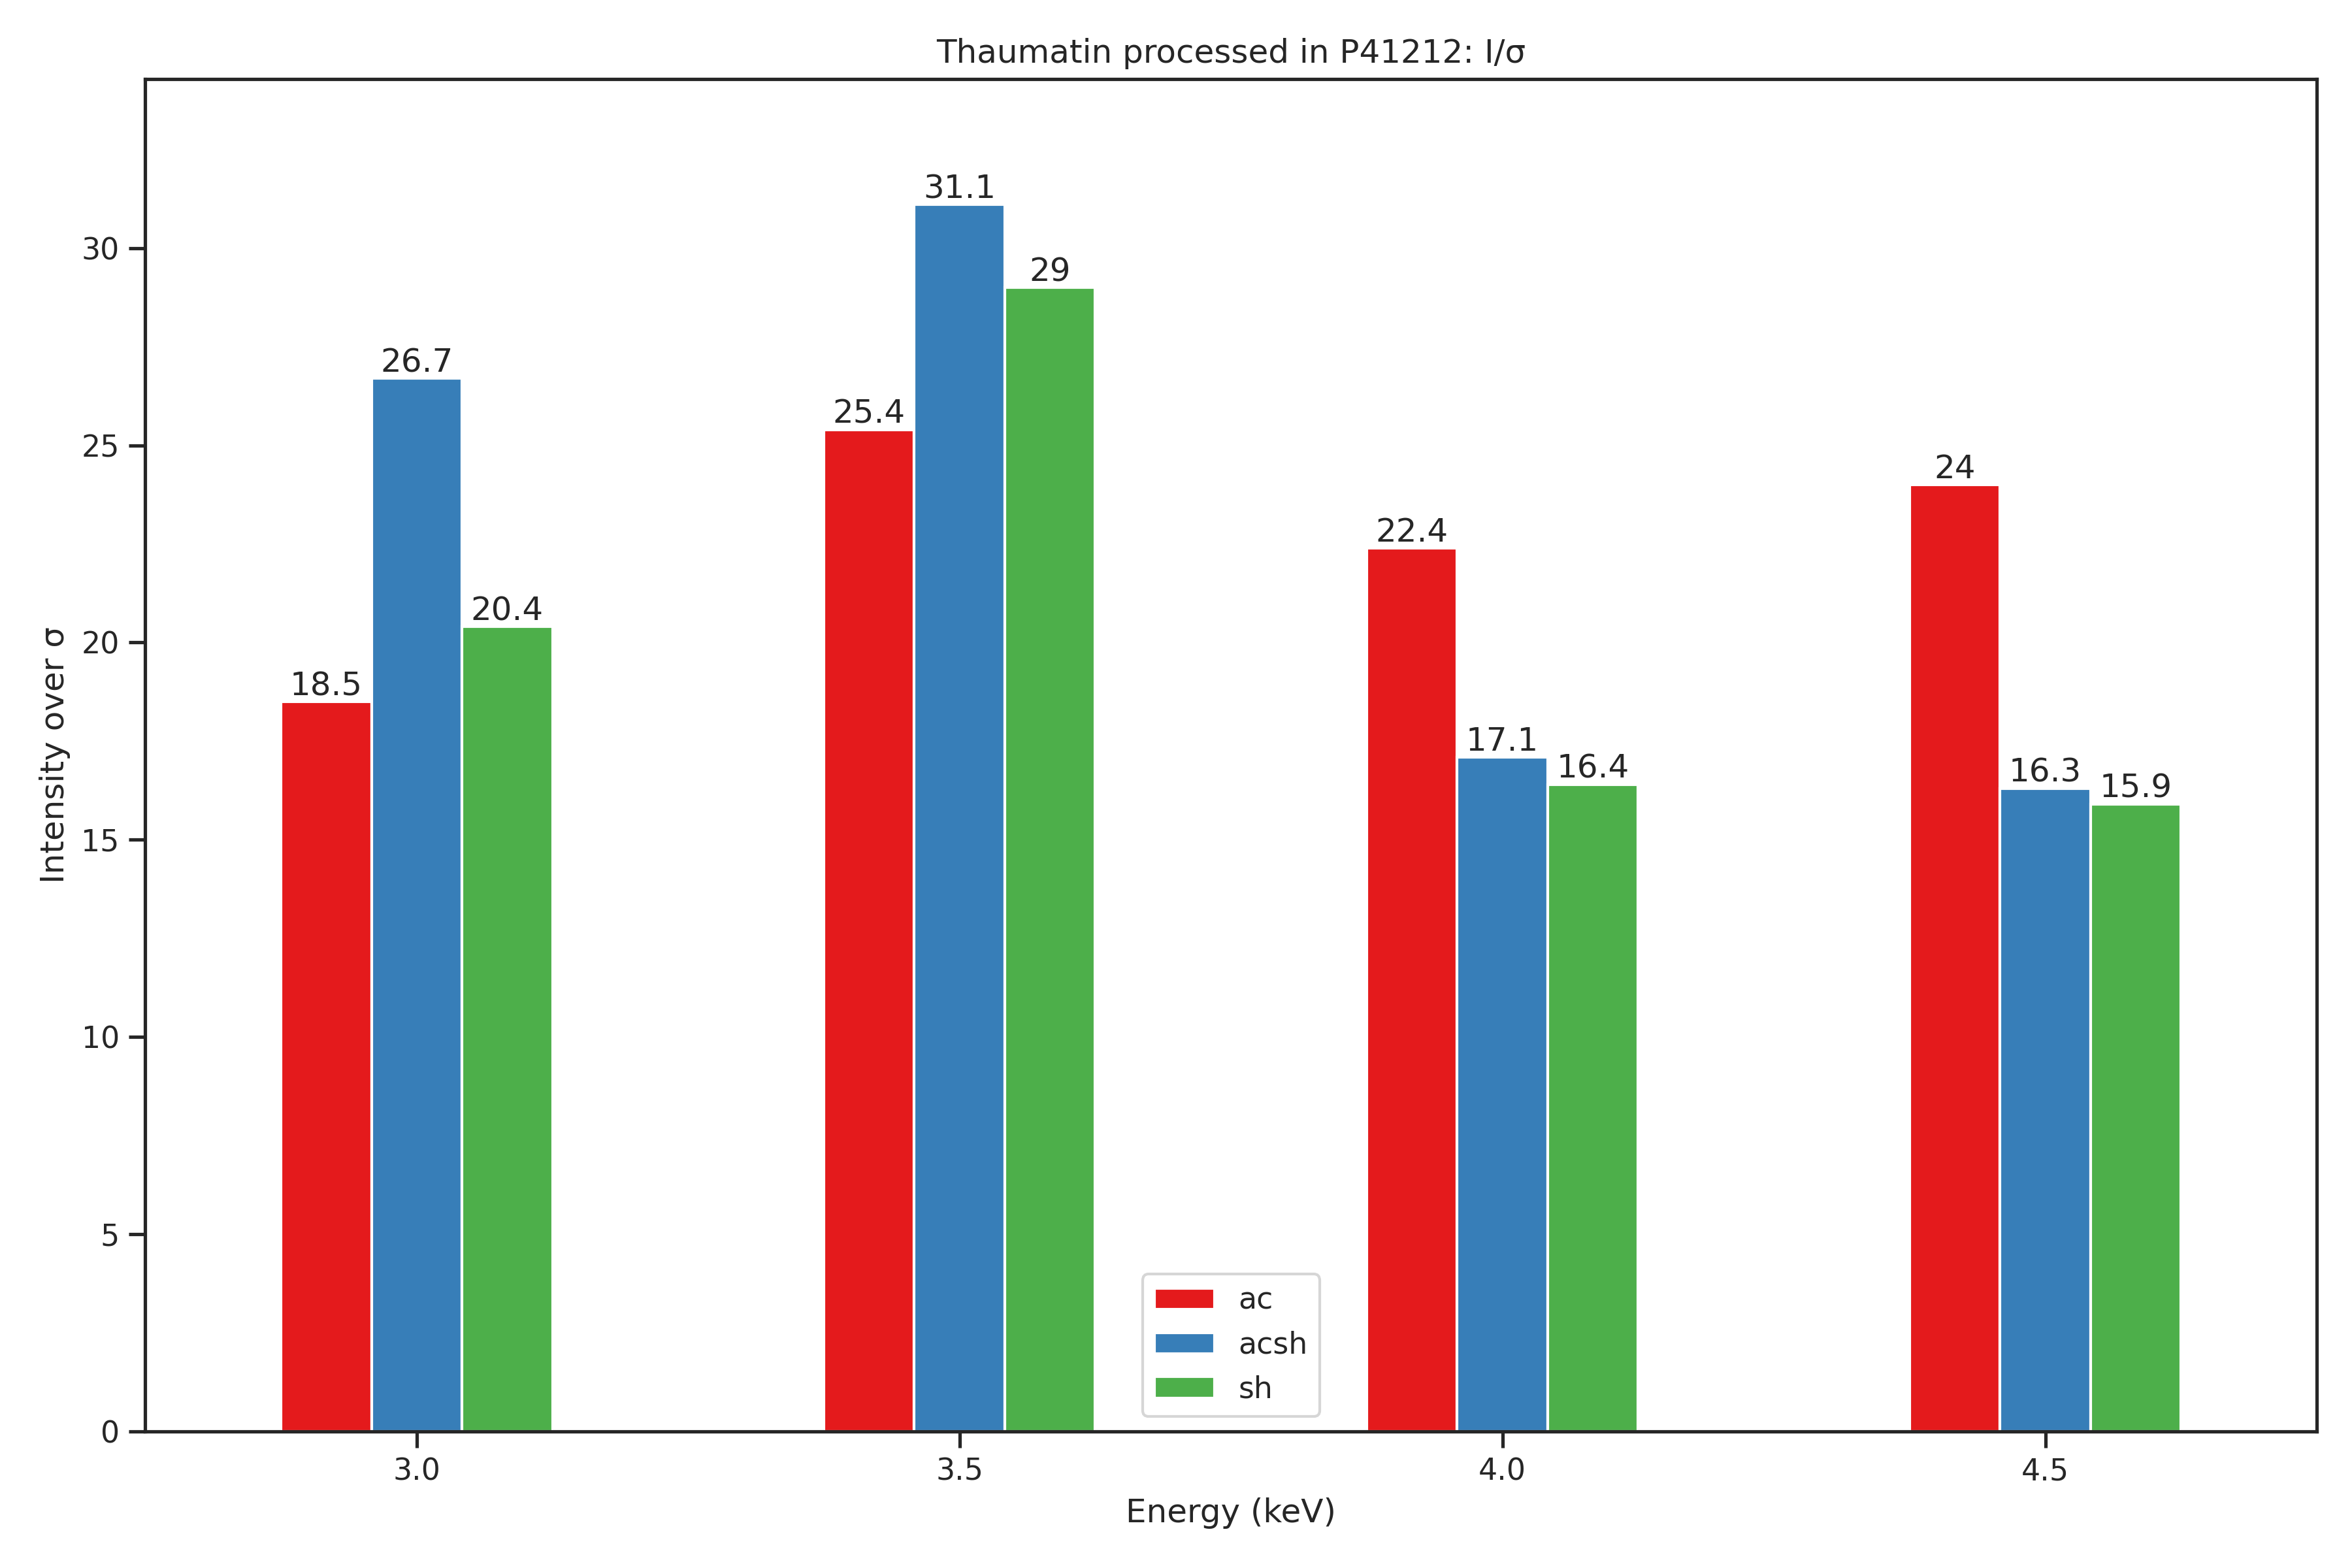
\includegraphics[width = 0.5\textwidth]{plots/exp0/thaum_Isig.png} & 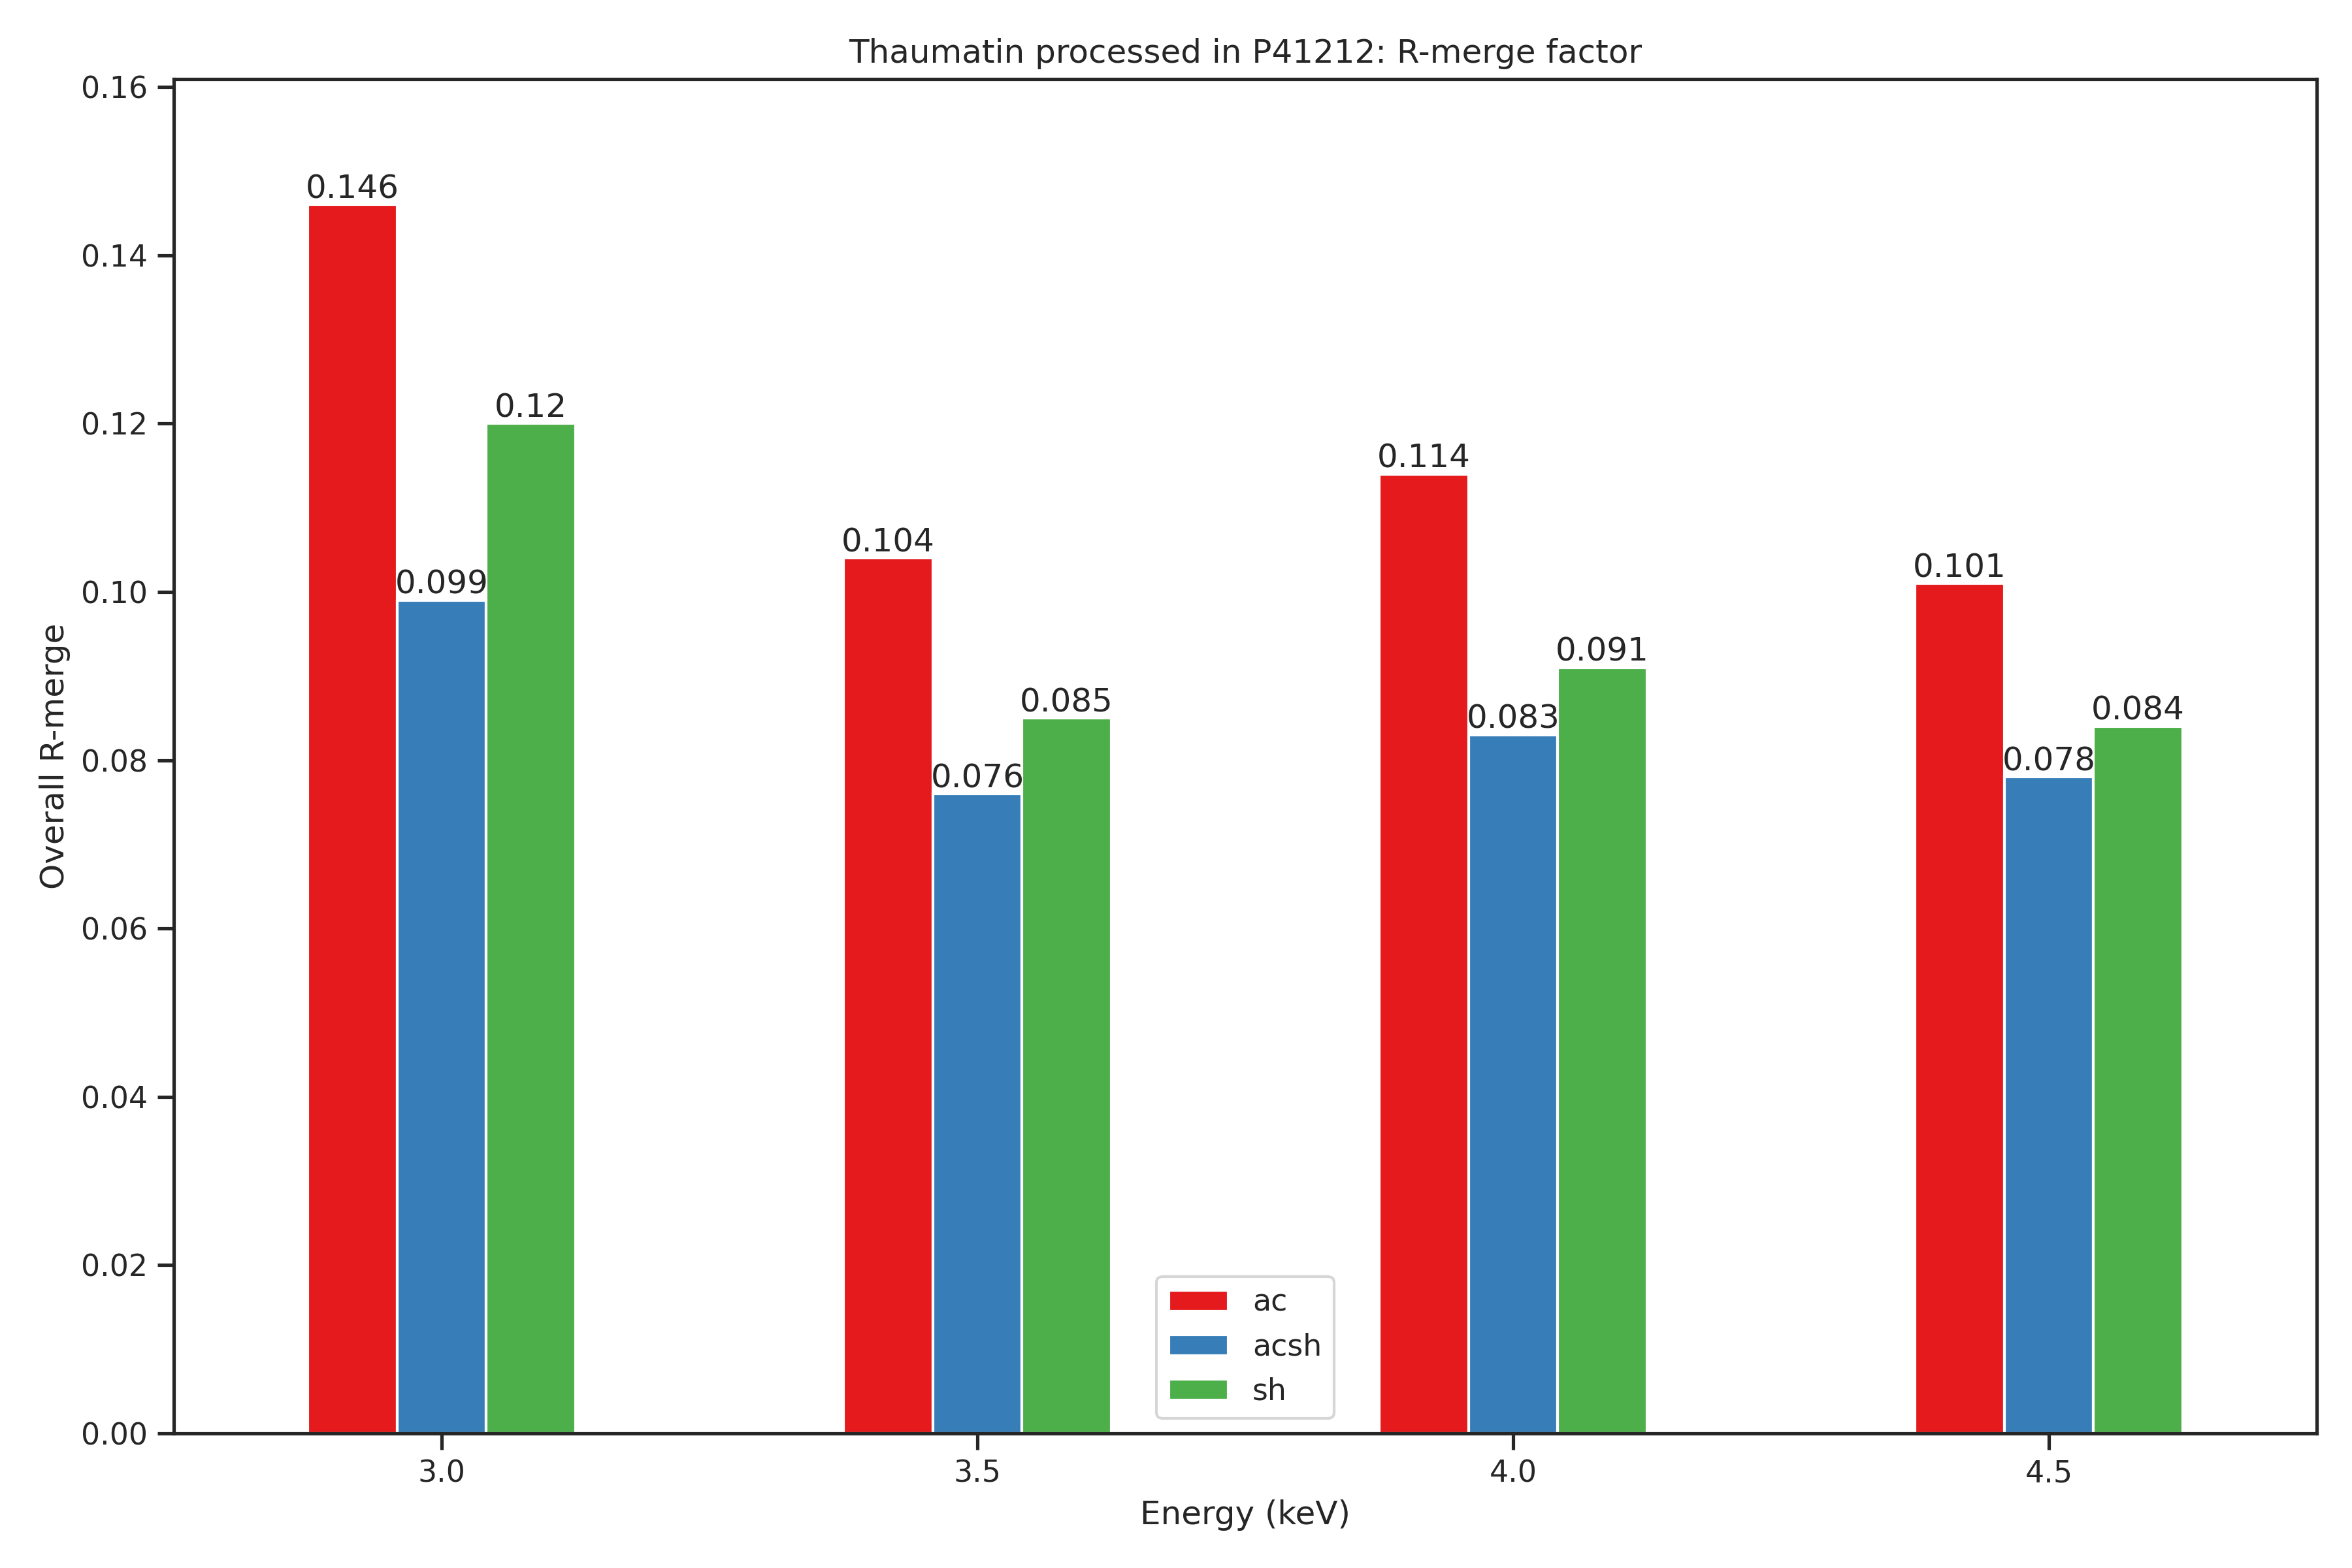
\includegraphics[width = 0.5\textwidth]{plots/exp0/thaum_rmerges.png}
    \end{tabular}
    \caption{Merging statistics for thaumatin crystal.}
    \label{fig:thaum1_stats}
\end{figure}


\newpage
%\section{Plots}

% TLYS 9 ANODE PEAKS
\begin{figure}
    \centering
    \begin{tabular}{cc}
        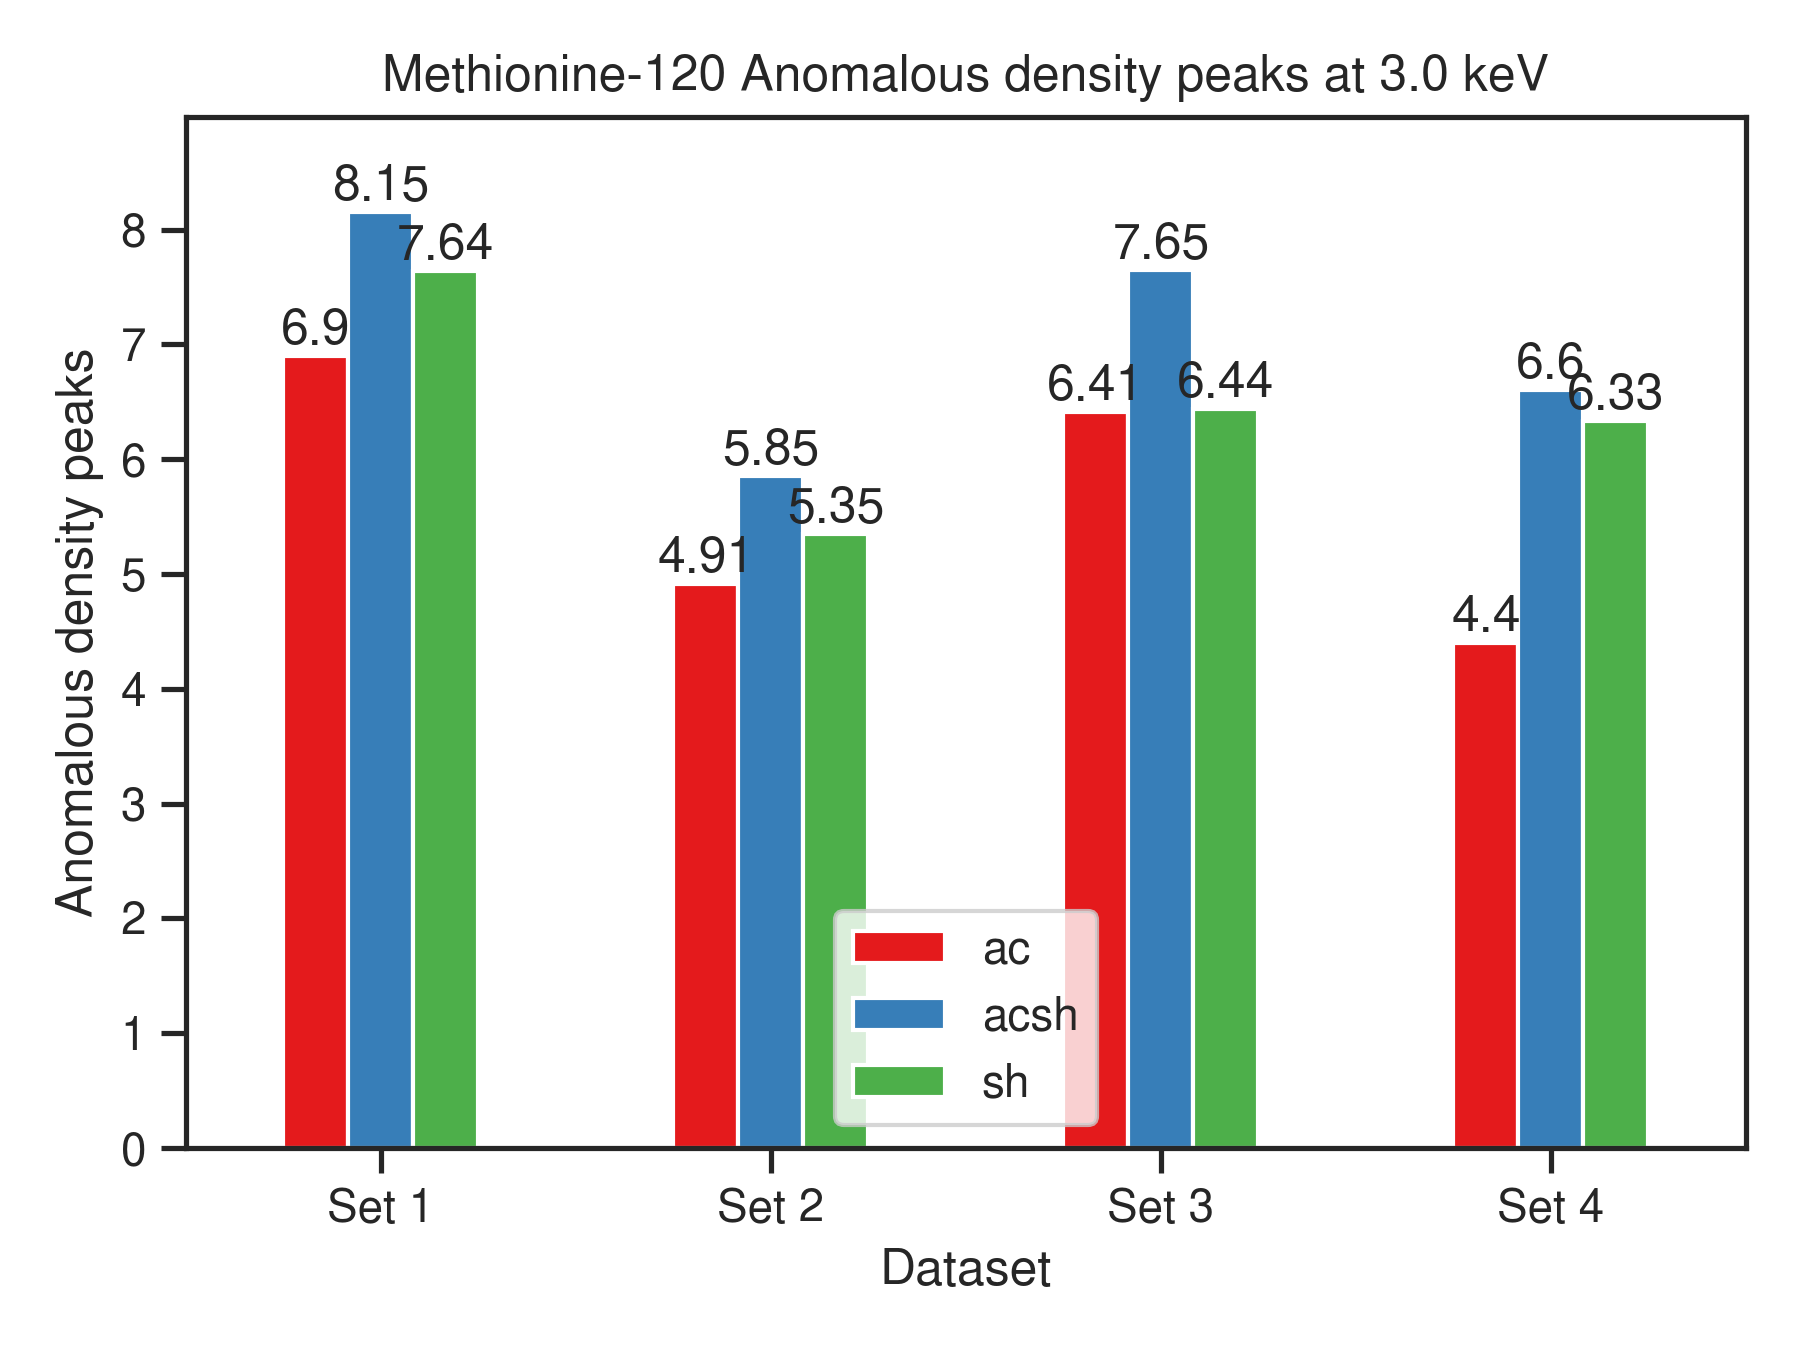
\includegraphics[width = 0.5\textwidth]{plots/exp1/tlys_9_P6122/peaks/3p0_met120_peaks.png} & 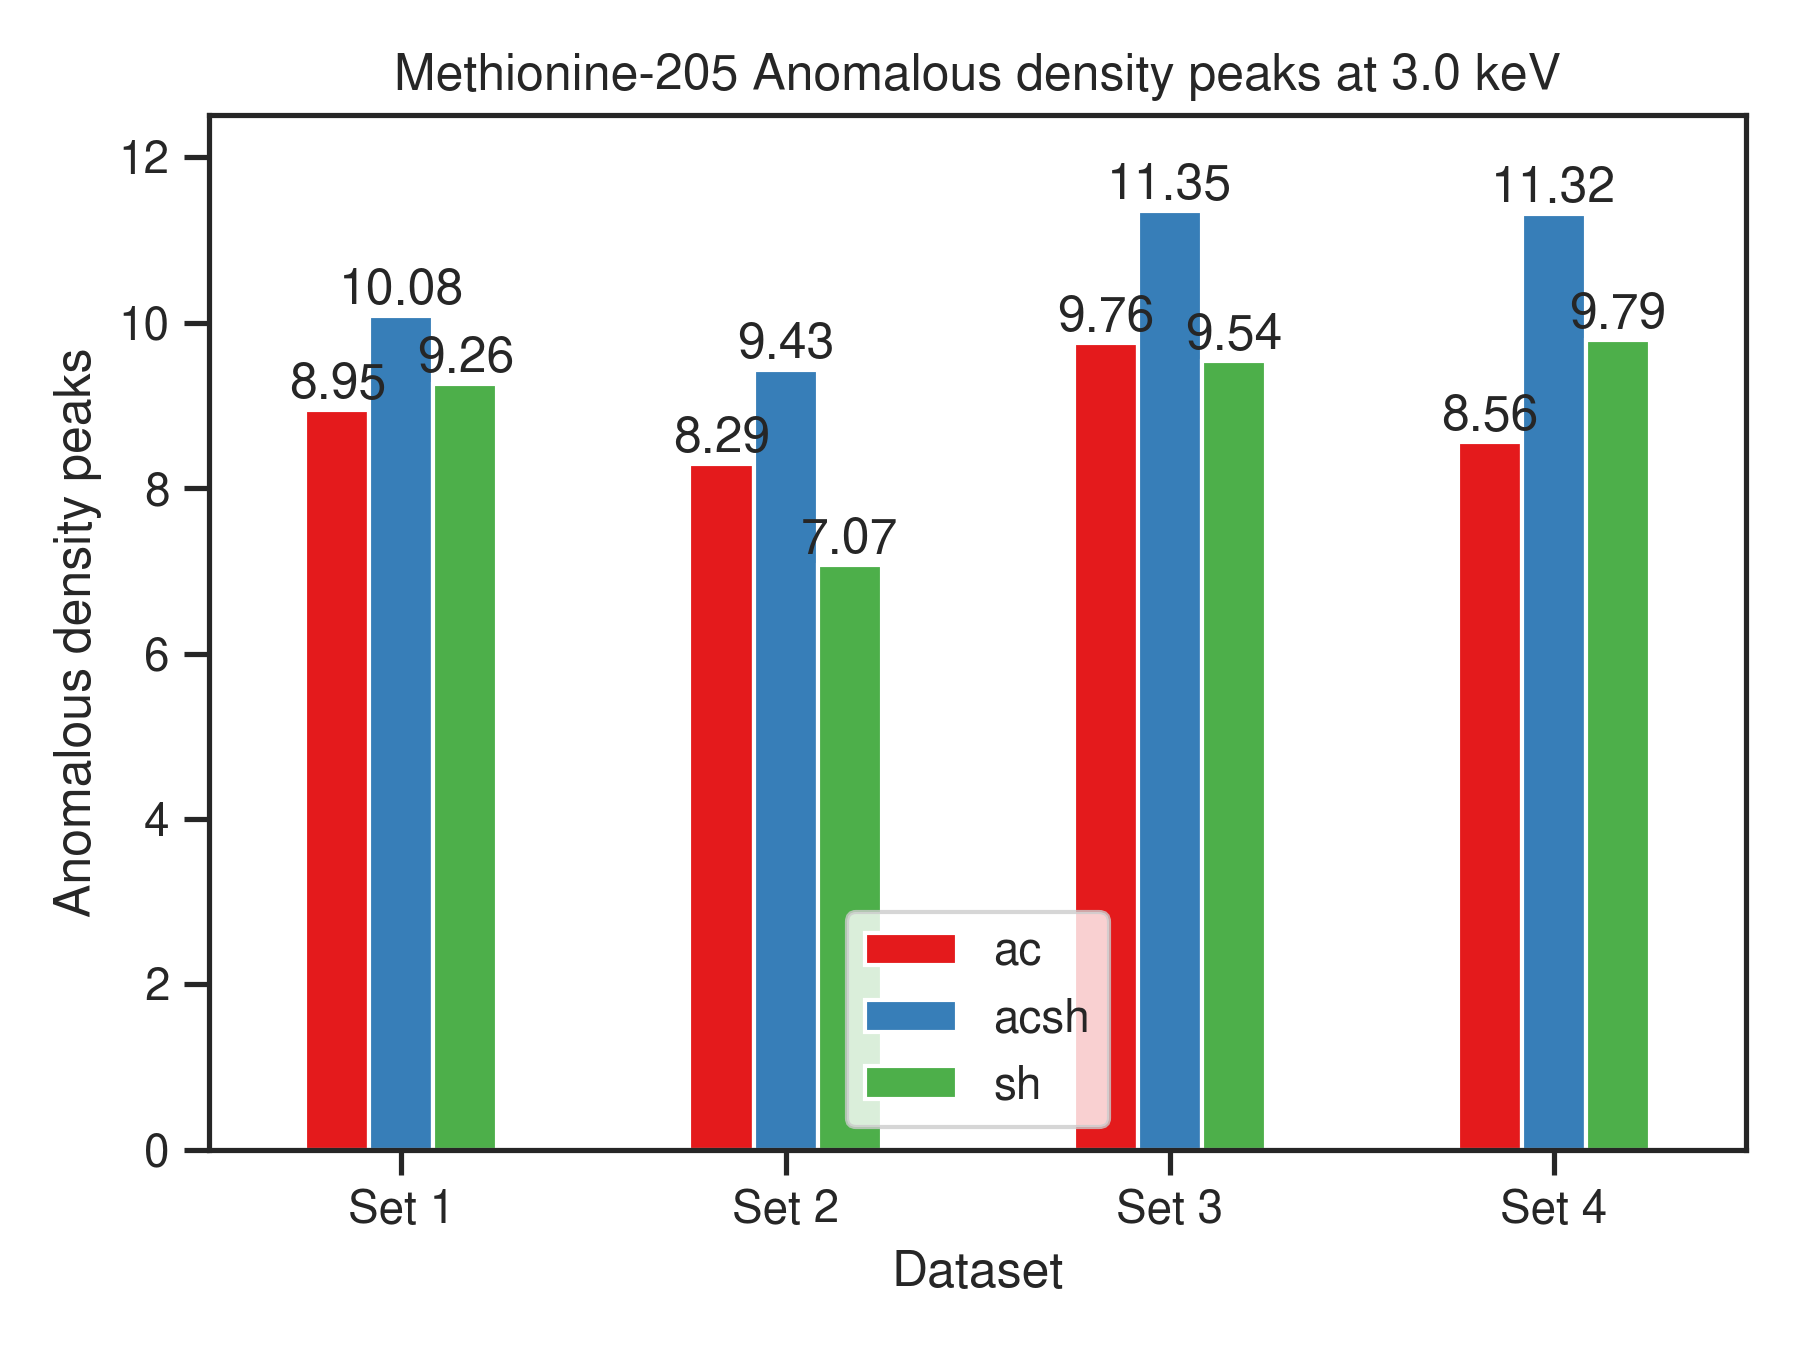
\includegraphics[width = 0.5\textwidth]{plots/exp1/tlys_9_P6122/peaks/3p0_met205_peaks.png}
    \end{tabular}
    \caption{Thermolysin 1: Anomalous density peaks of methionine groups at 3.0 \unit{keV}.}
    \label{fig:tlys9_met_peaks_3p0}
\end{figure}

\begin{figure}
    \centering
    \begin{tabular}{cc}
        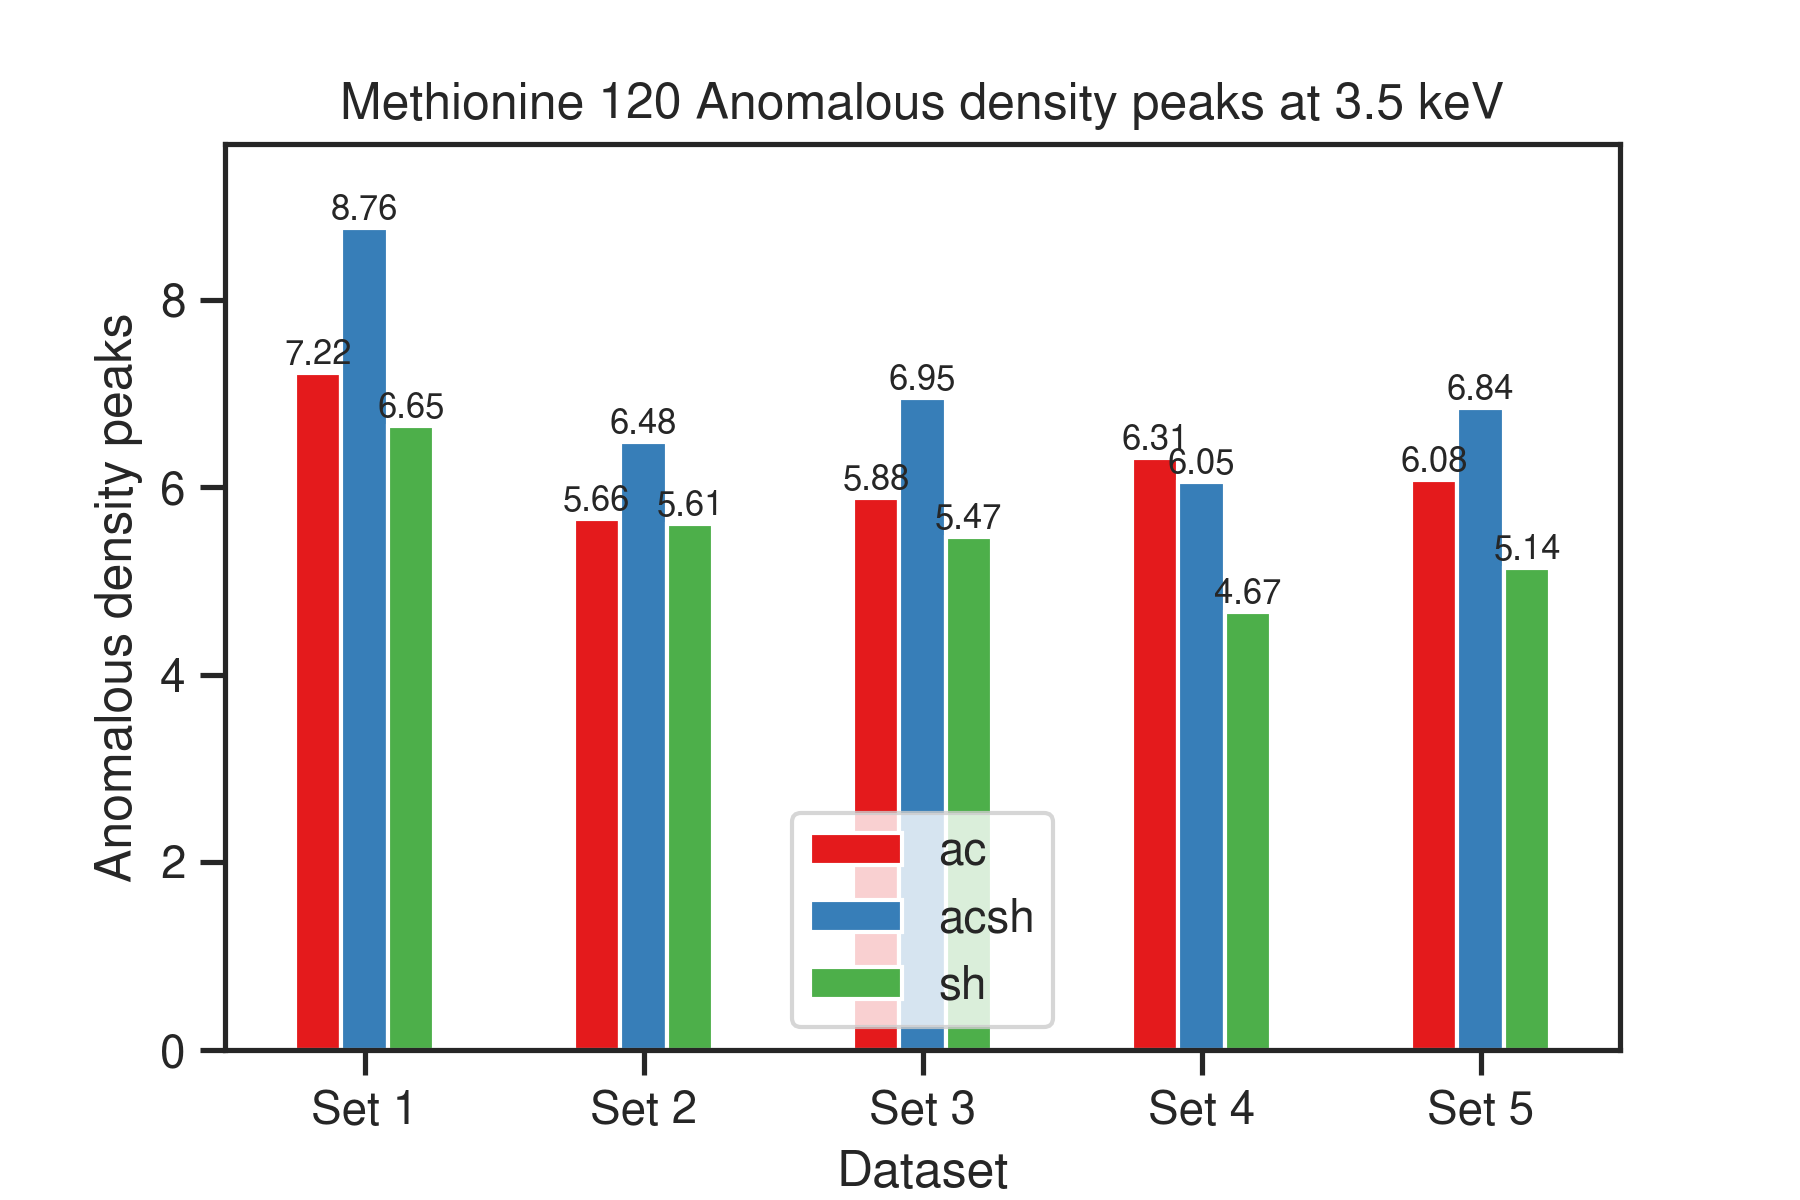
\includegraphics[width = 0.5\textwidth]{plots/exp1/tlys_9_P6122/peaks/3p5_met120_peaks.png} & 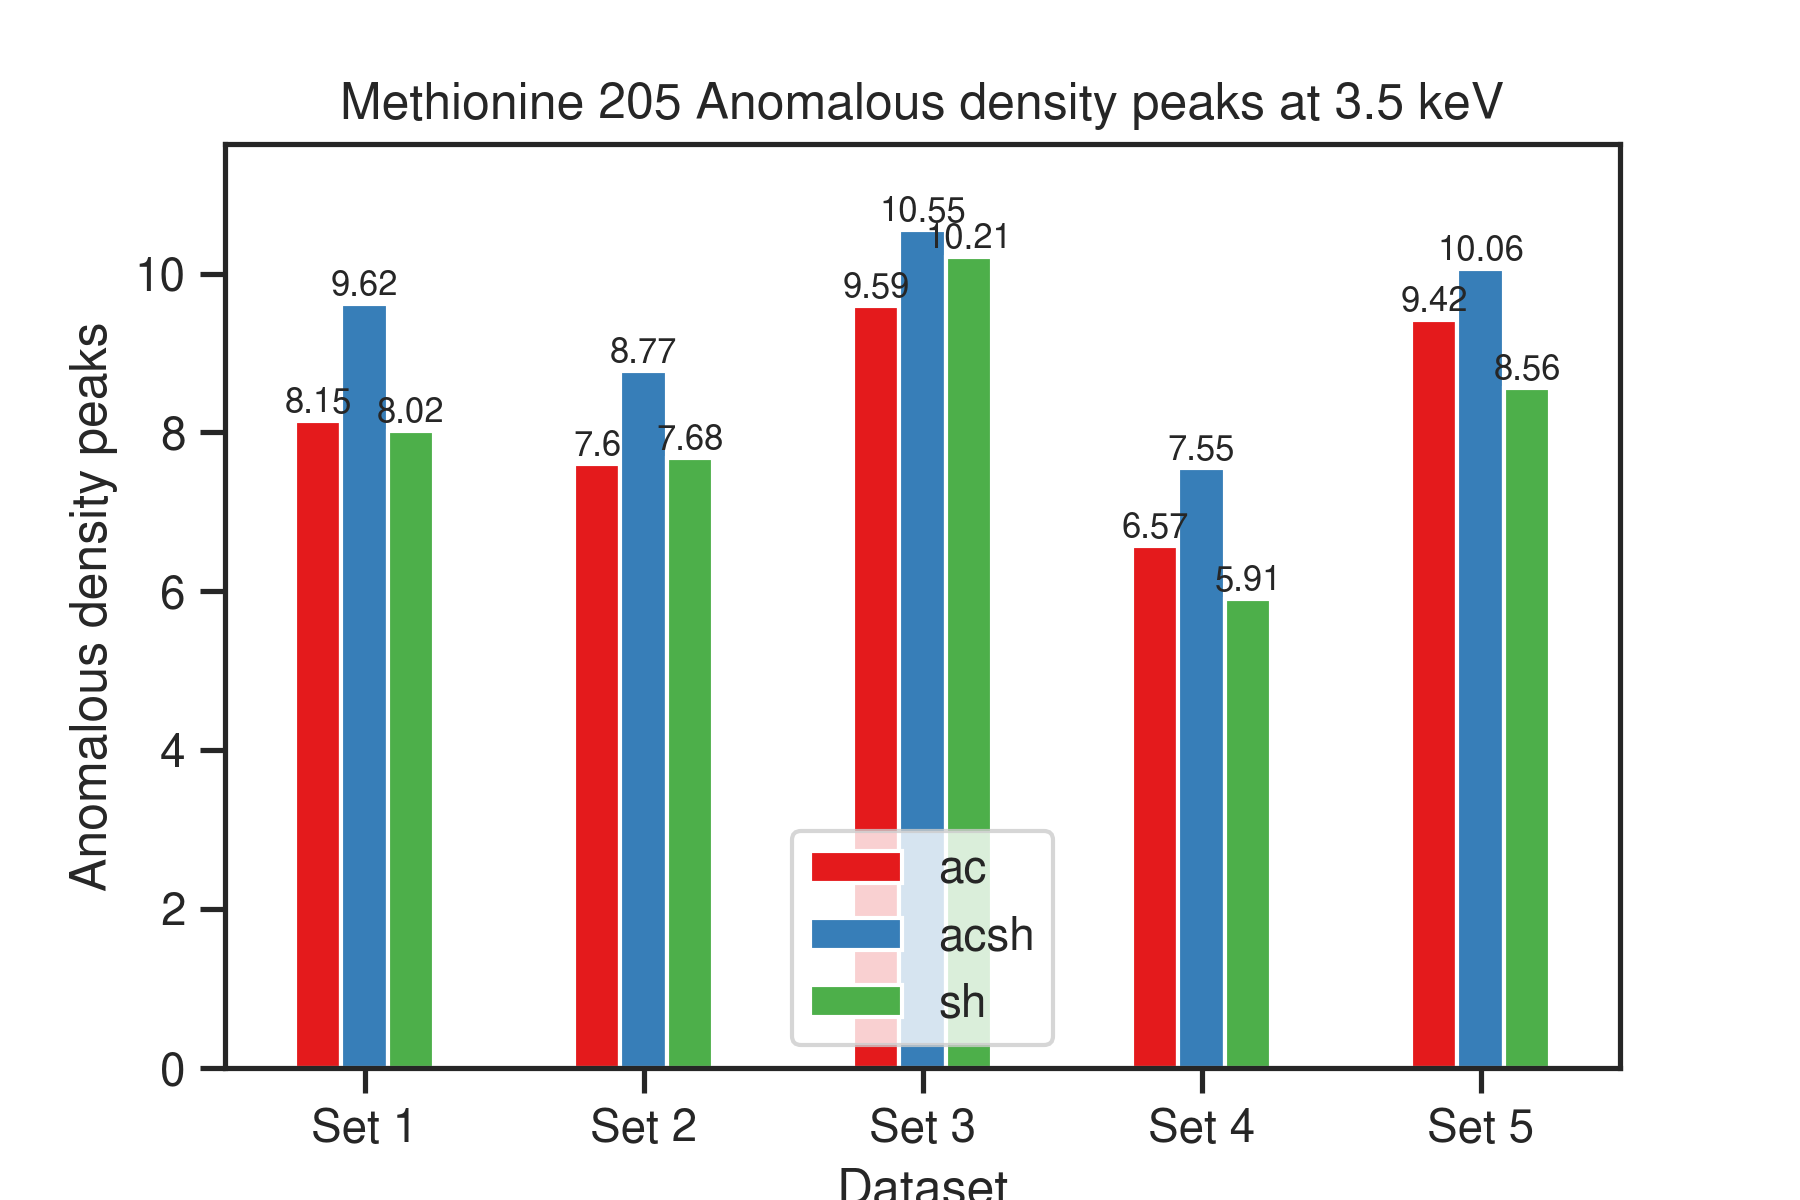
\includegraphics[width = 0.5\textwidth]{plots/exp1/tlys_9_P6122/peaks/3p5_met205_peaks.png}
    \end{tabular}
    \caption{Thermolysin 1: Anomalous density peaks of methionine groups at 3.5 \unit{keV}.}
    \label{fig:tlys9_met_peaks_3p5}
\end{figure}

\begin{figure}
    \centering
    \begin{tabular}{cc}
        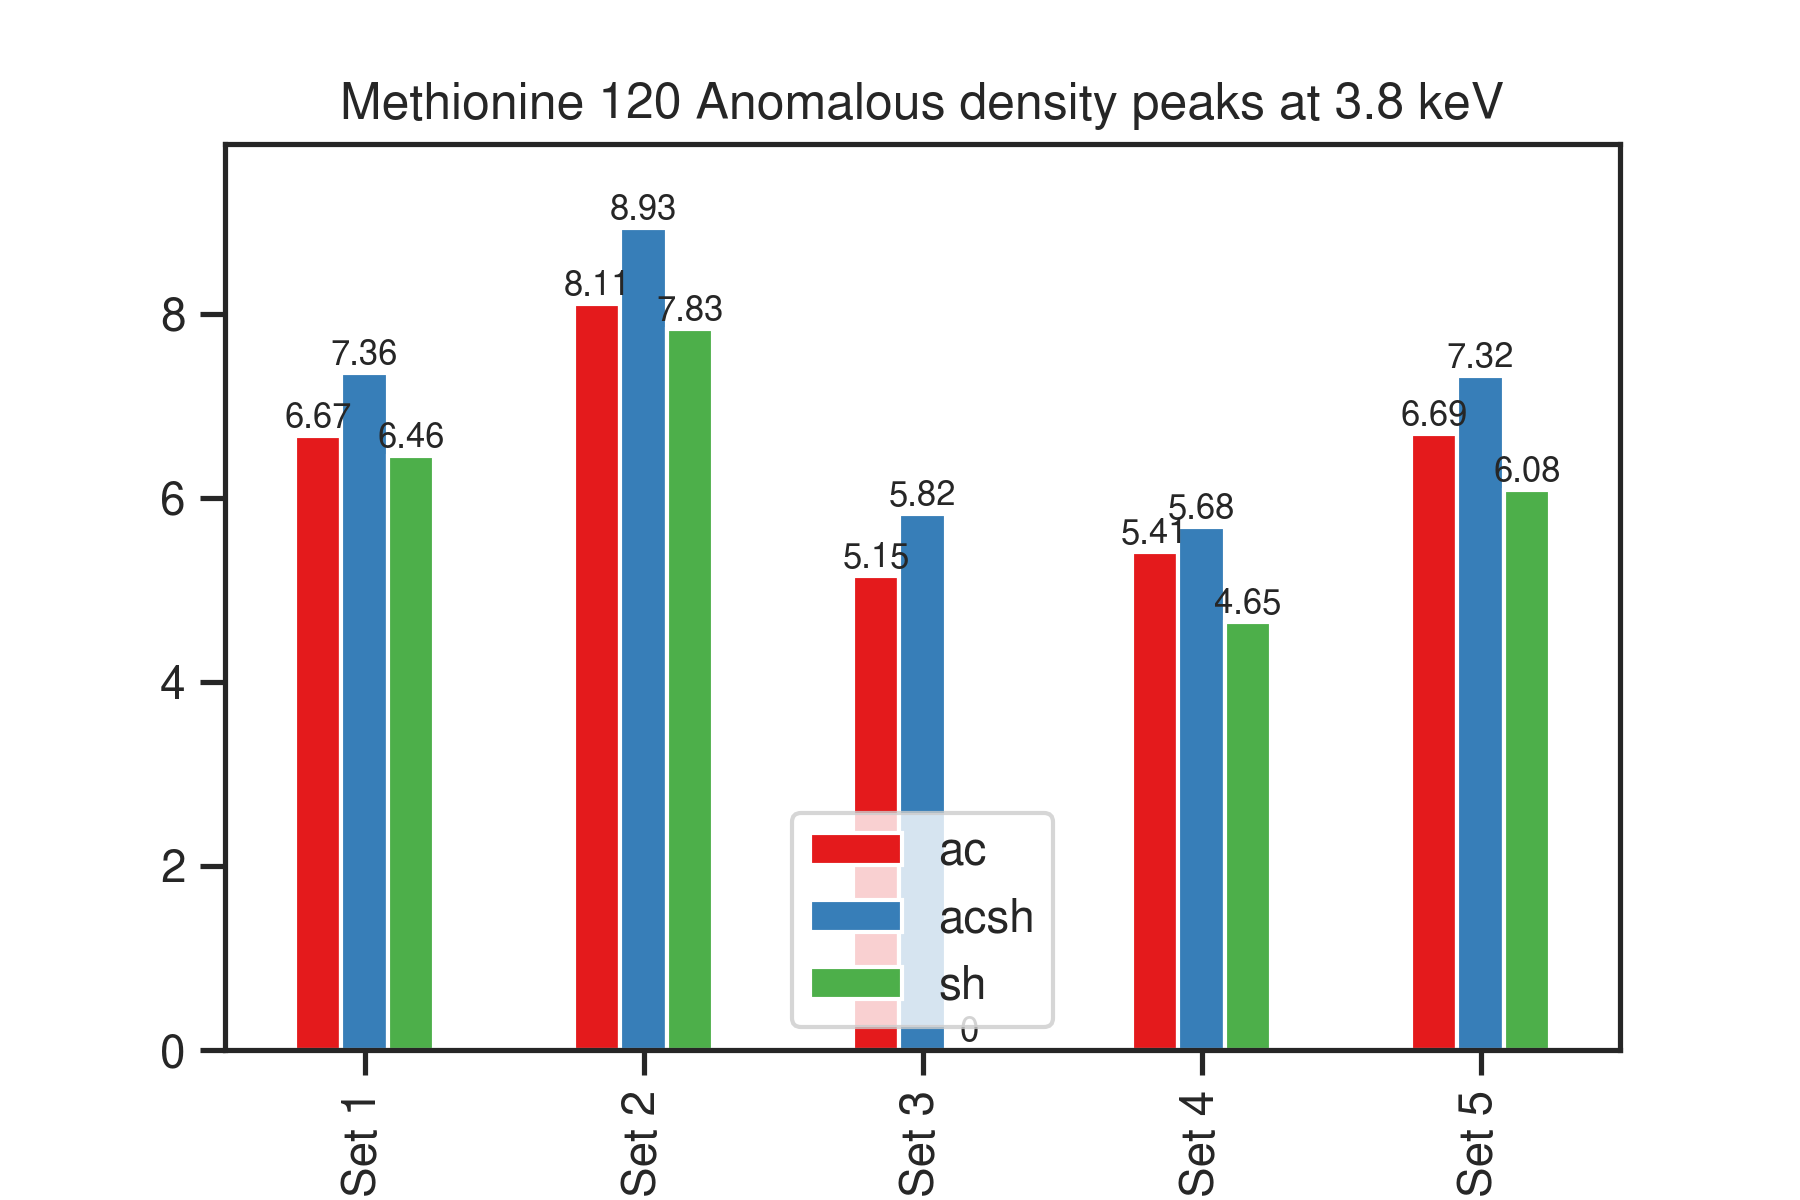
\includegraphics[width = 0.5\textwidth]{plots/exp1/tlys_9_P6122/peaks/3p8_met120_peaks.png} & 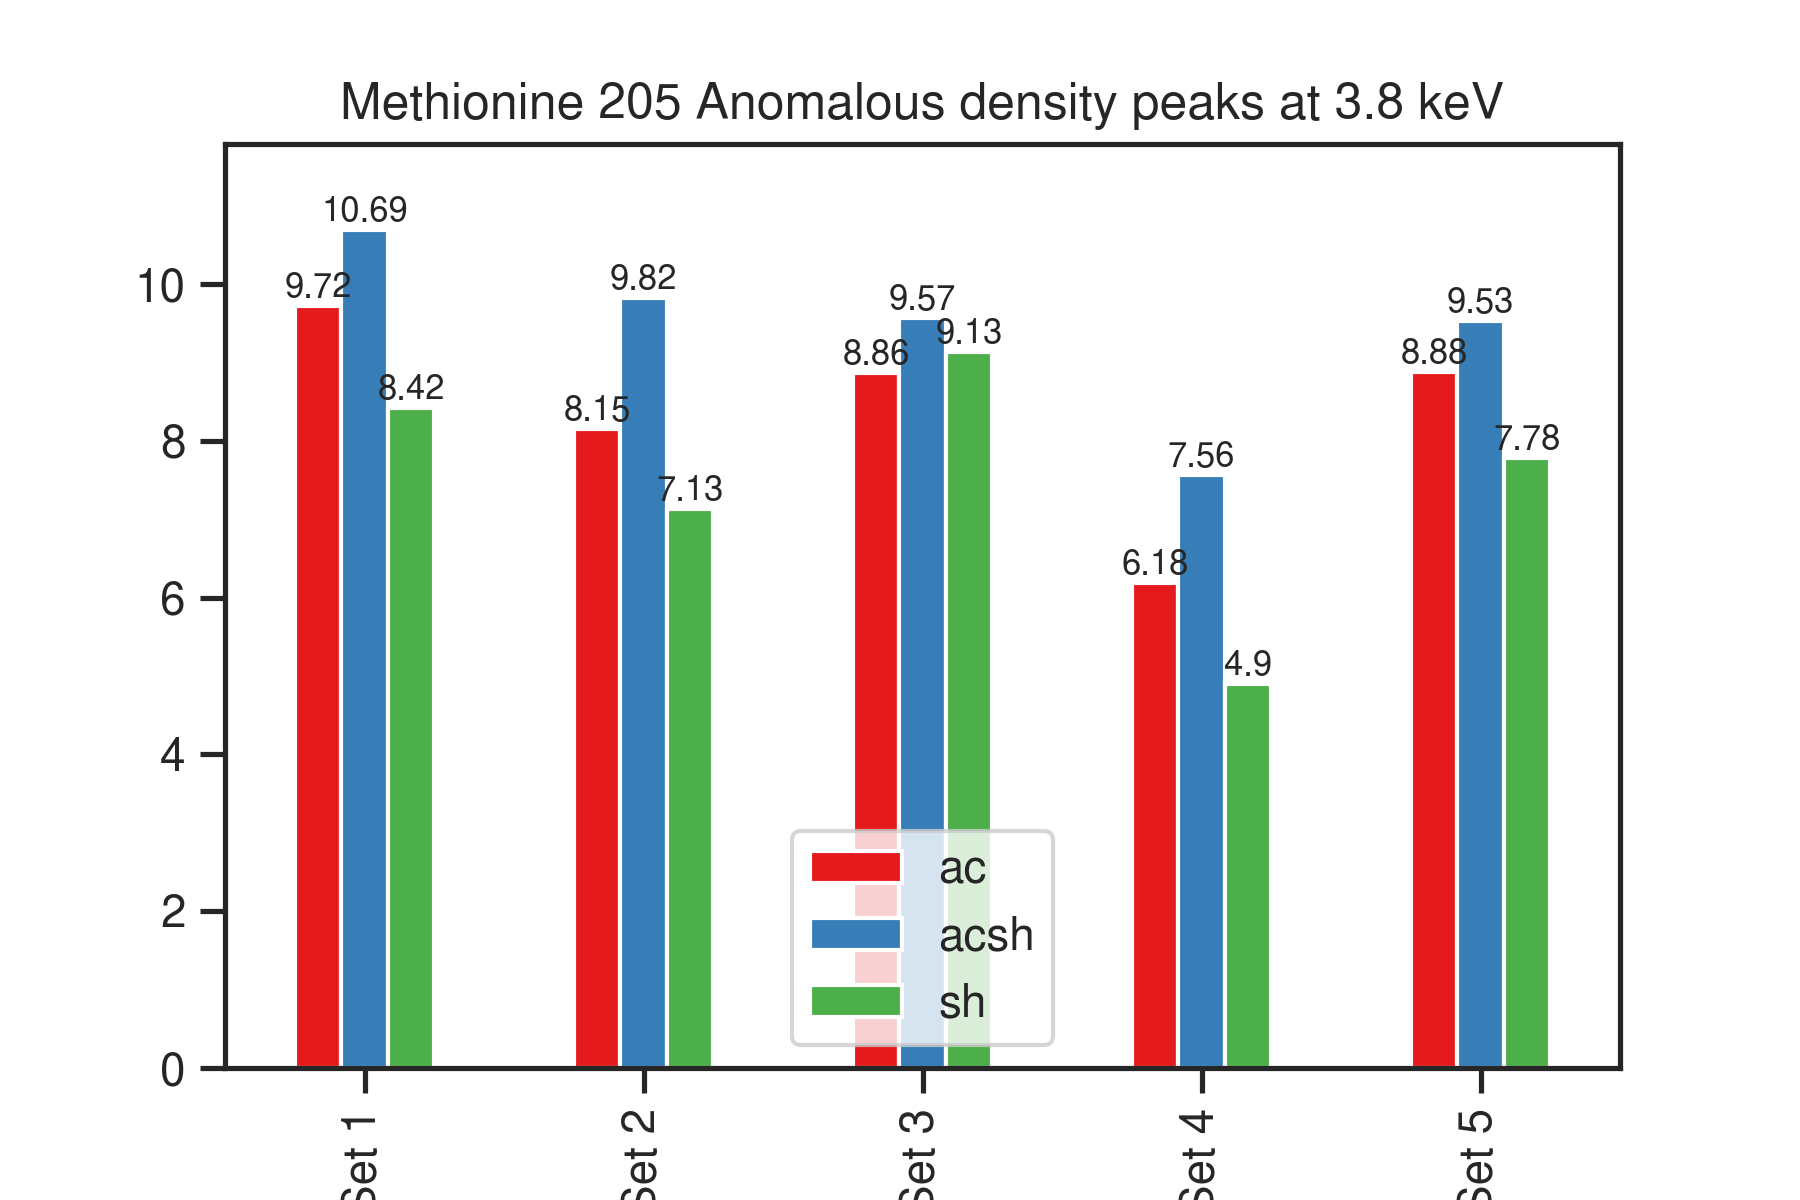
\includegraphics[width = 0.5\textwidth]{plots/exp1/tlys_9_P6122/peaks/3p8_met205_peaks.png}
    \end{tabular}
    \caption{Thermolysin 1: Anomalous density peaks of methionine groups at 3.8 \unit{keV}.}
    \label{fig:tlys9_met_peaks_3p8}
\end{figure}

\begin{figure}
    \centering
    \begin{tabular}{cc}
        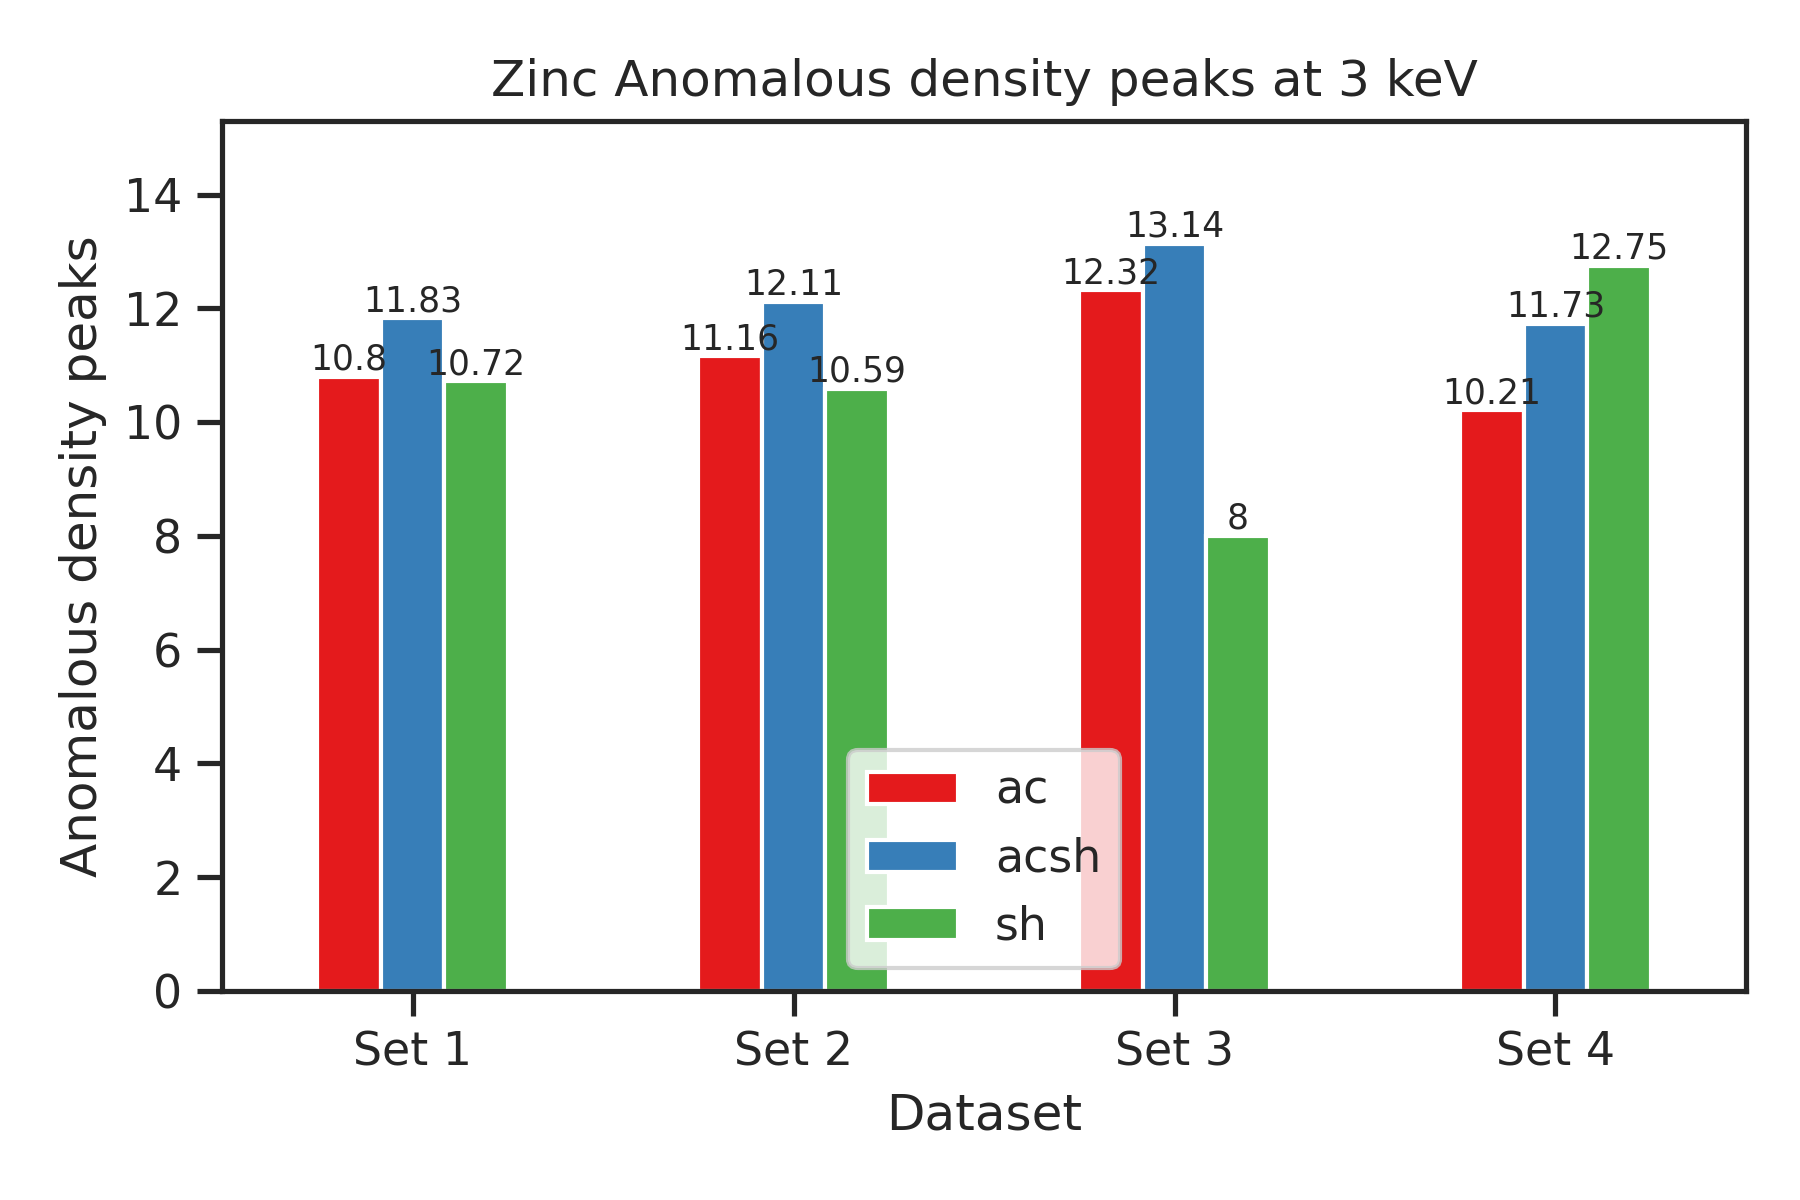
\includegraphics[width = 0.5\textwidth]{plots/exp1/tlys_2_P6122/peaks/3p0_zn_2Dbar.png} & 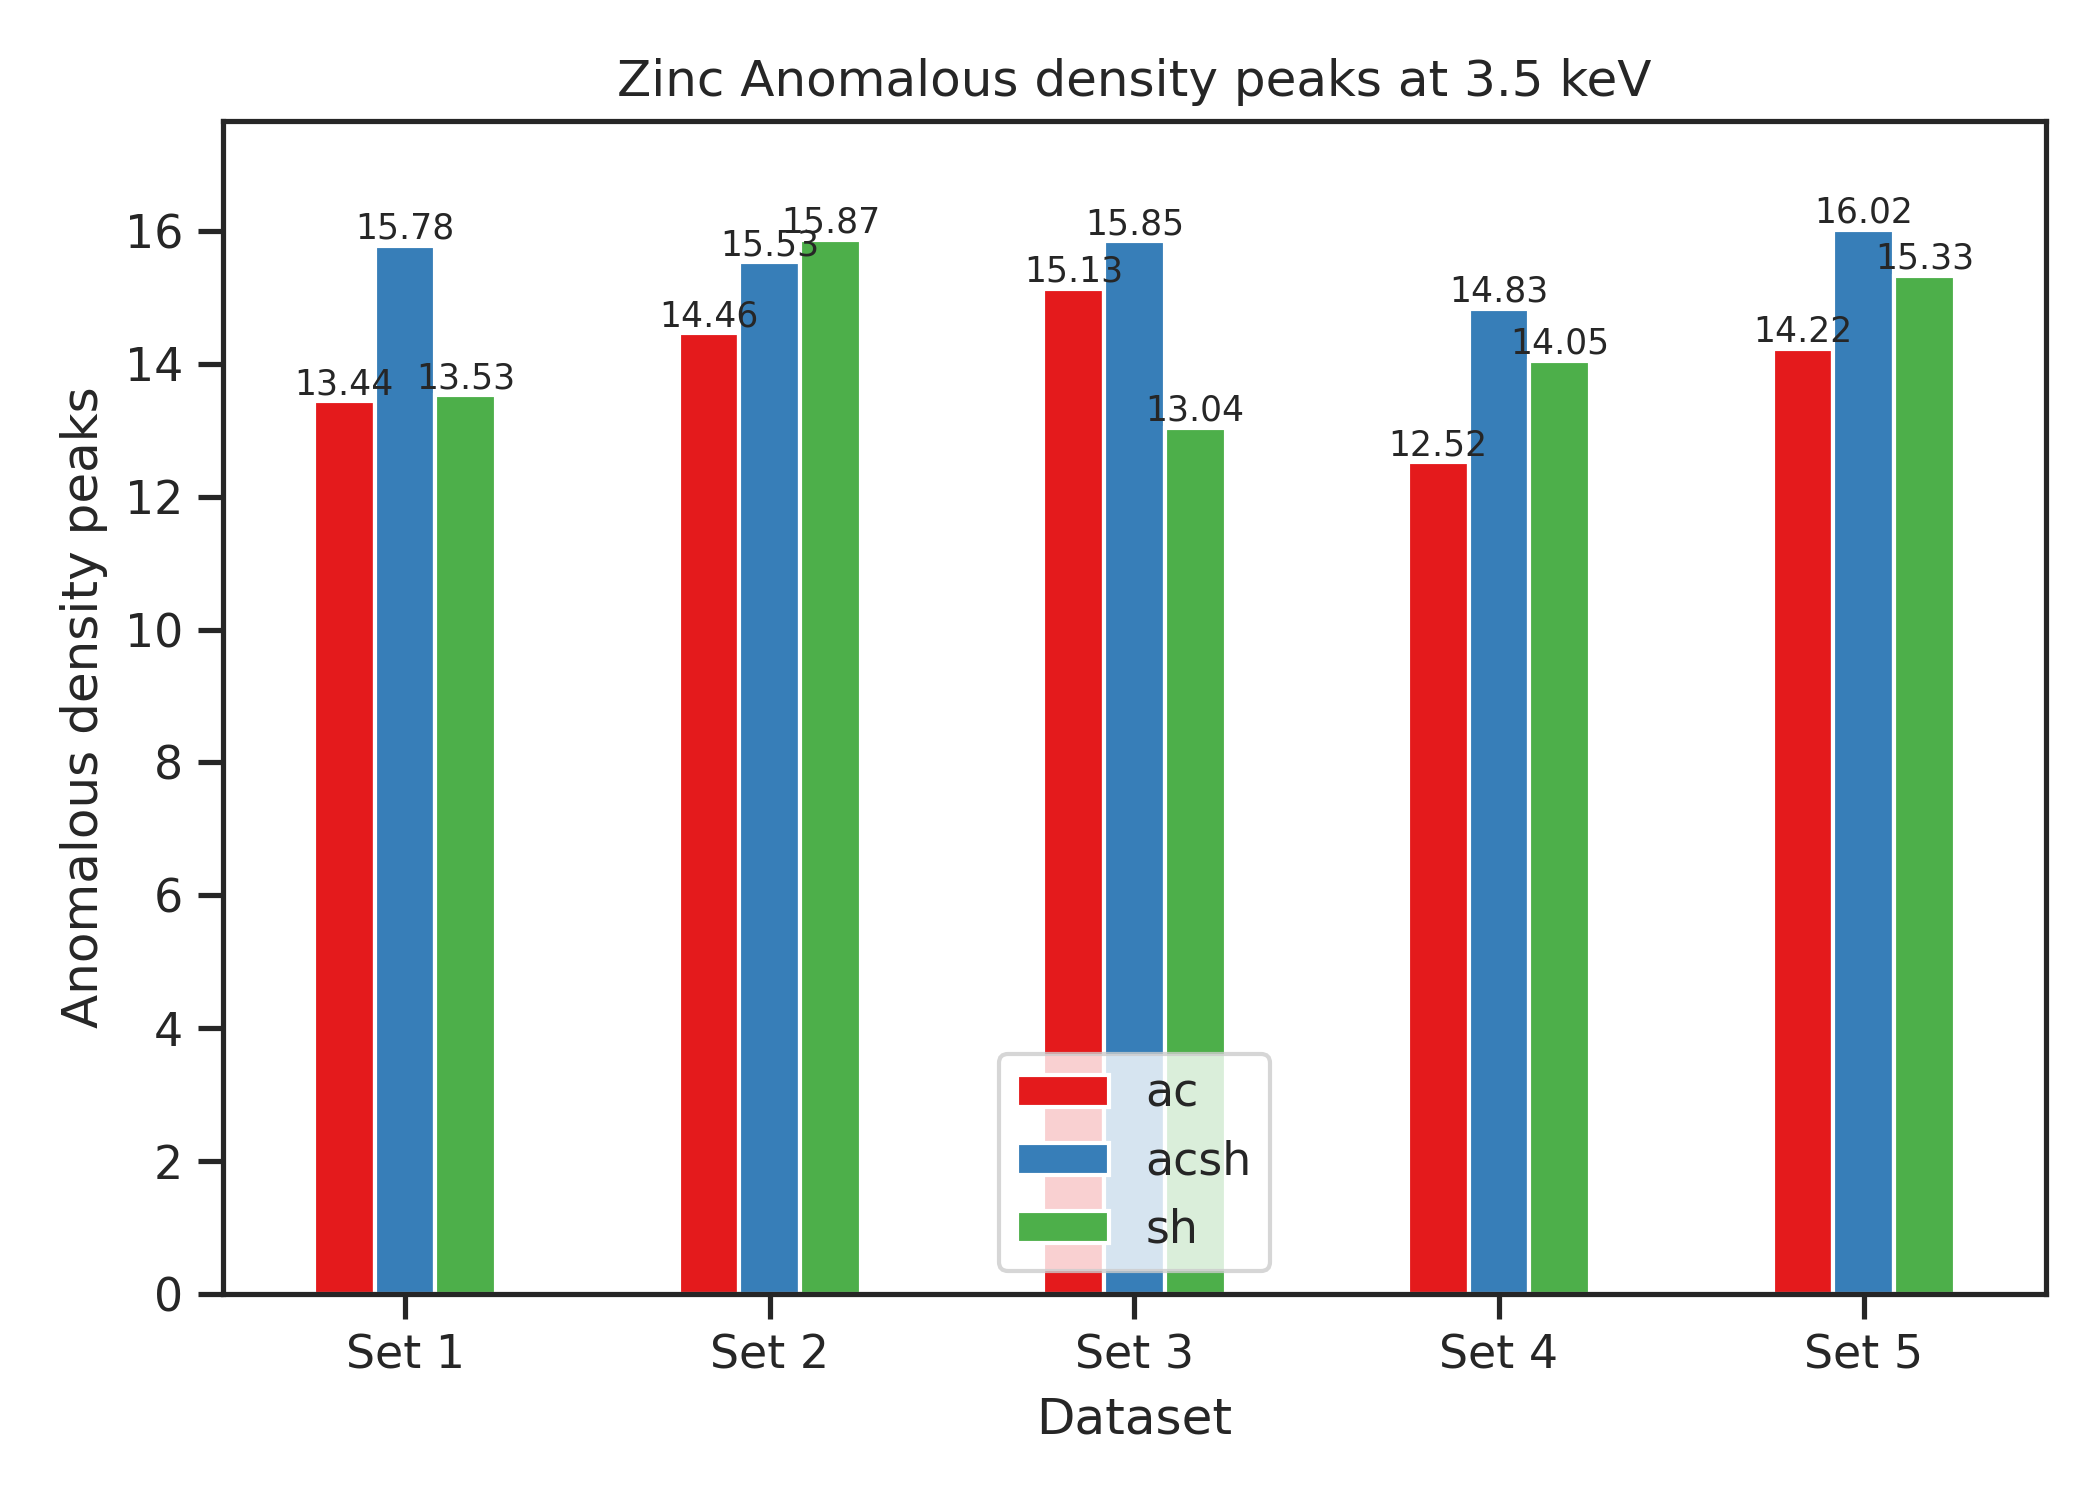
\includegraphics[width = 0.5\textwidth]{plots/exp1/tlys_2_P6122/peaks/3p5_zn_2Dbar.png}
    \end{tabular}
    \caption{Thermolysin 1: Anomalous density peaks of Zinc at 3.0 and 3.5 \unit{keV}.}
    \label{fig:tlys9_zn_peaks_3p0_3p5}
\end{figure}

\begin{figure}
    \centering
    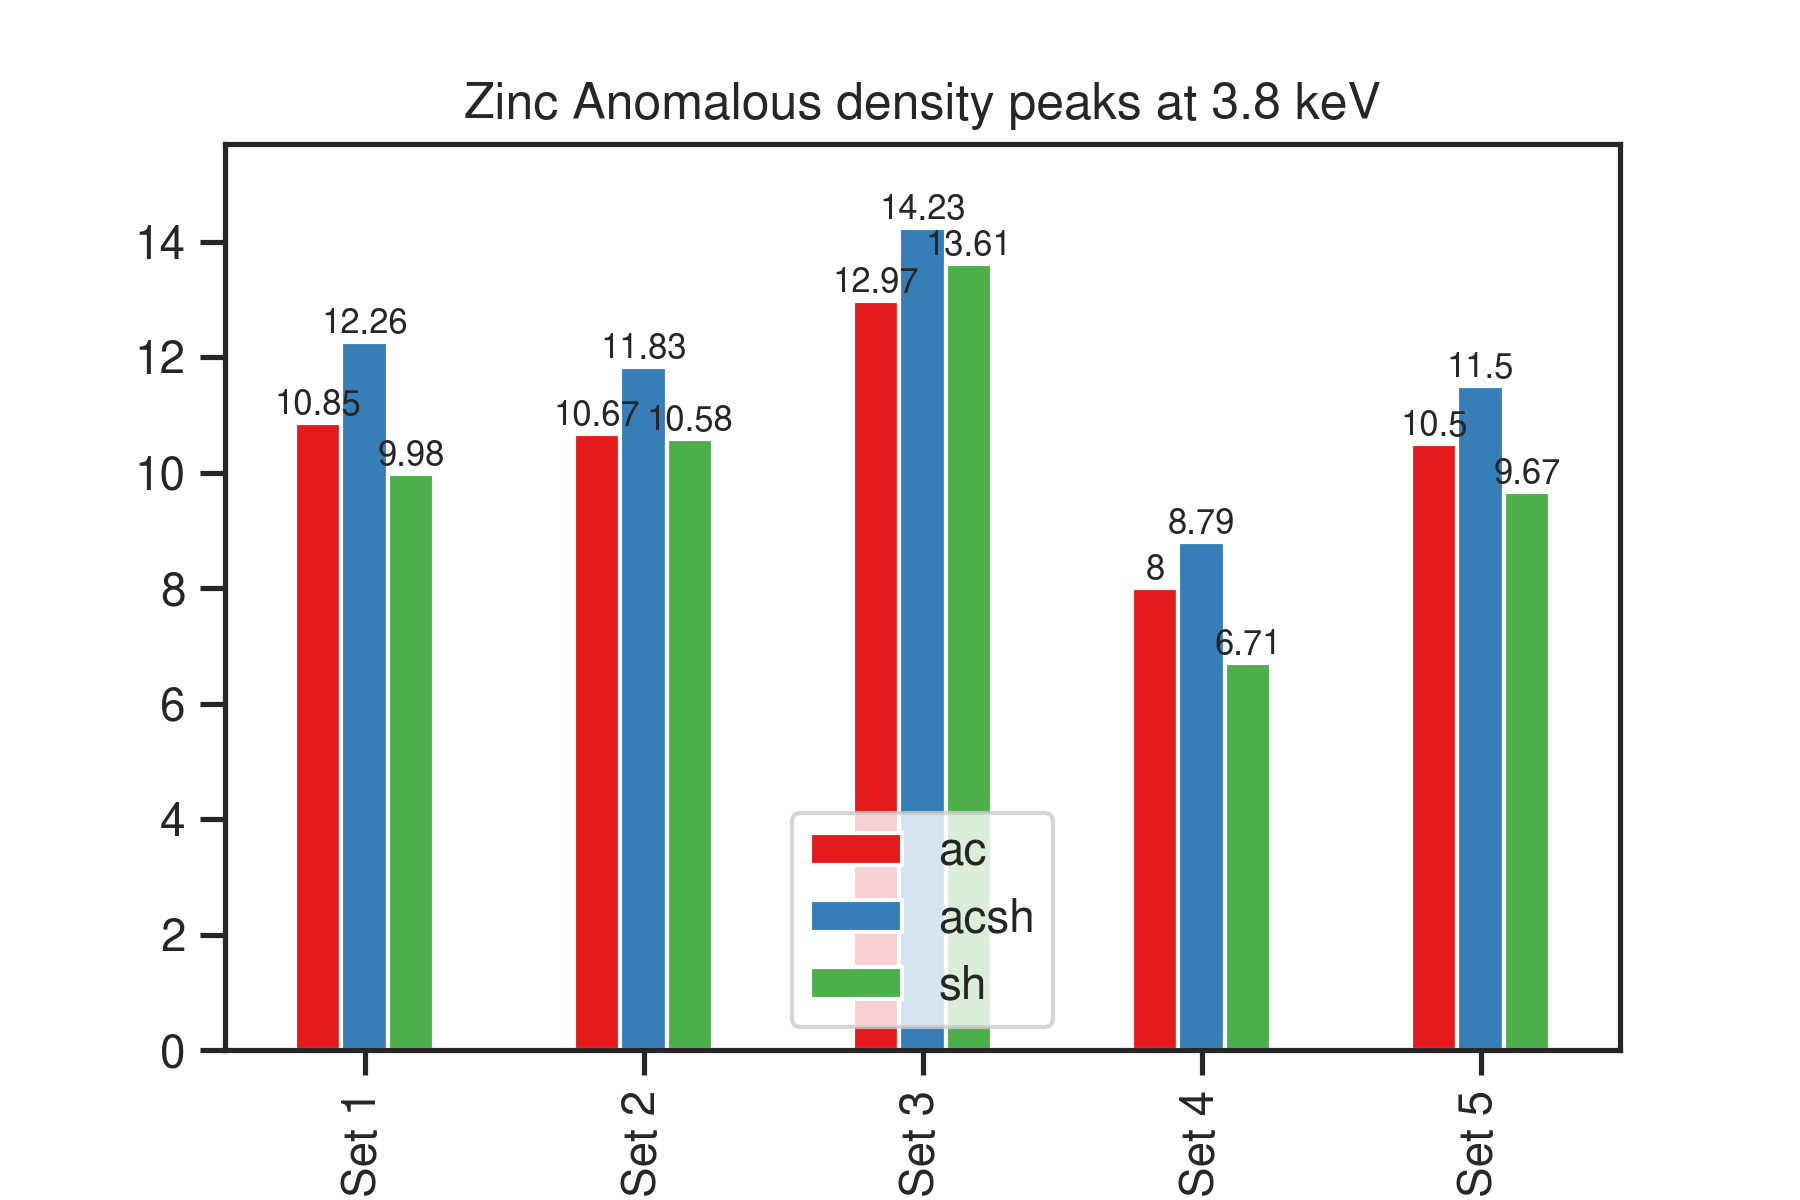
\includegraphics[width = 0.5\textwidth]{plots/exp1/tlys_9_P6122/peaks/3p8_zn405_peaks.png}
    \caption{Thermolysin 1: Anomalous density peaks of Zinc at 3.8 \unit{keV}.}
    \label{fig:tlys9_zn_peaks_3p8}
\end{figure}



% TLYS 2 ANODE PEAKS
\begin{figure}
    \centering
    \begin{tabular}{cc}
        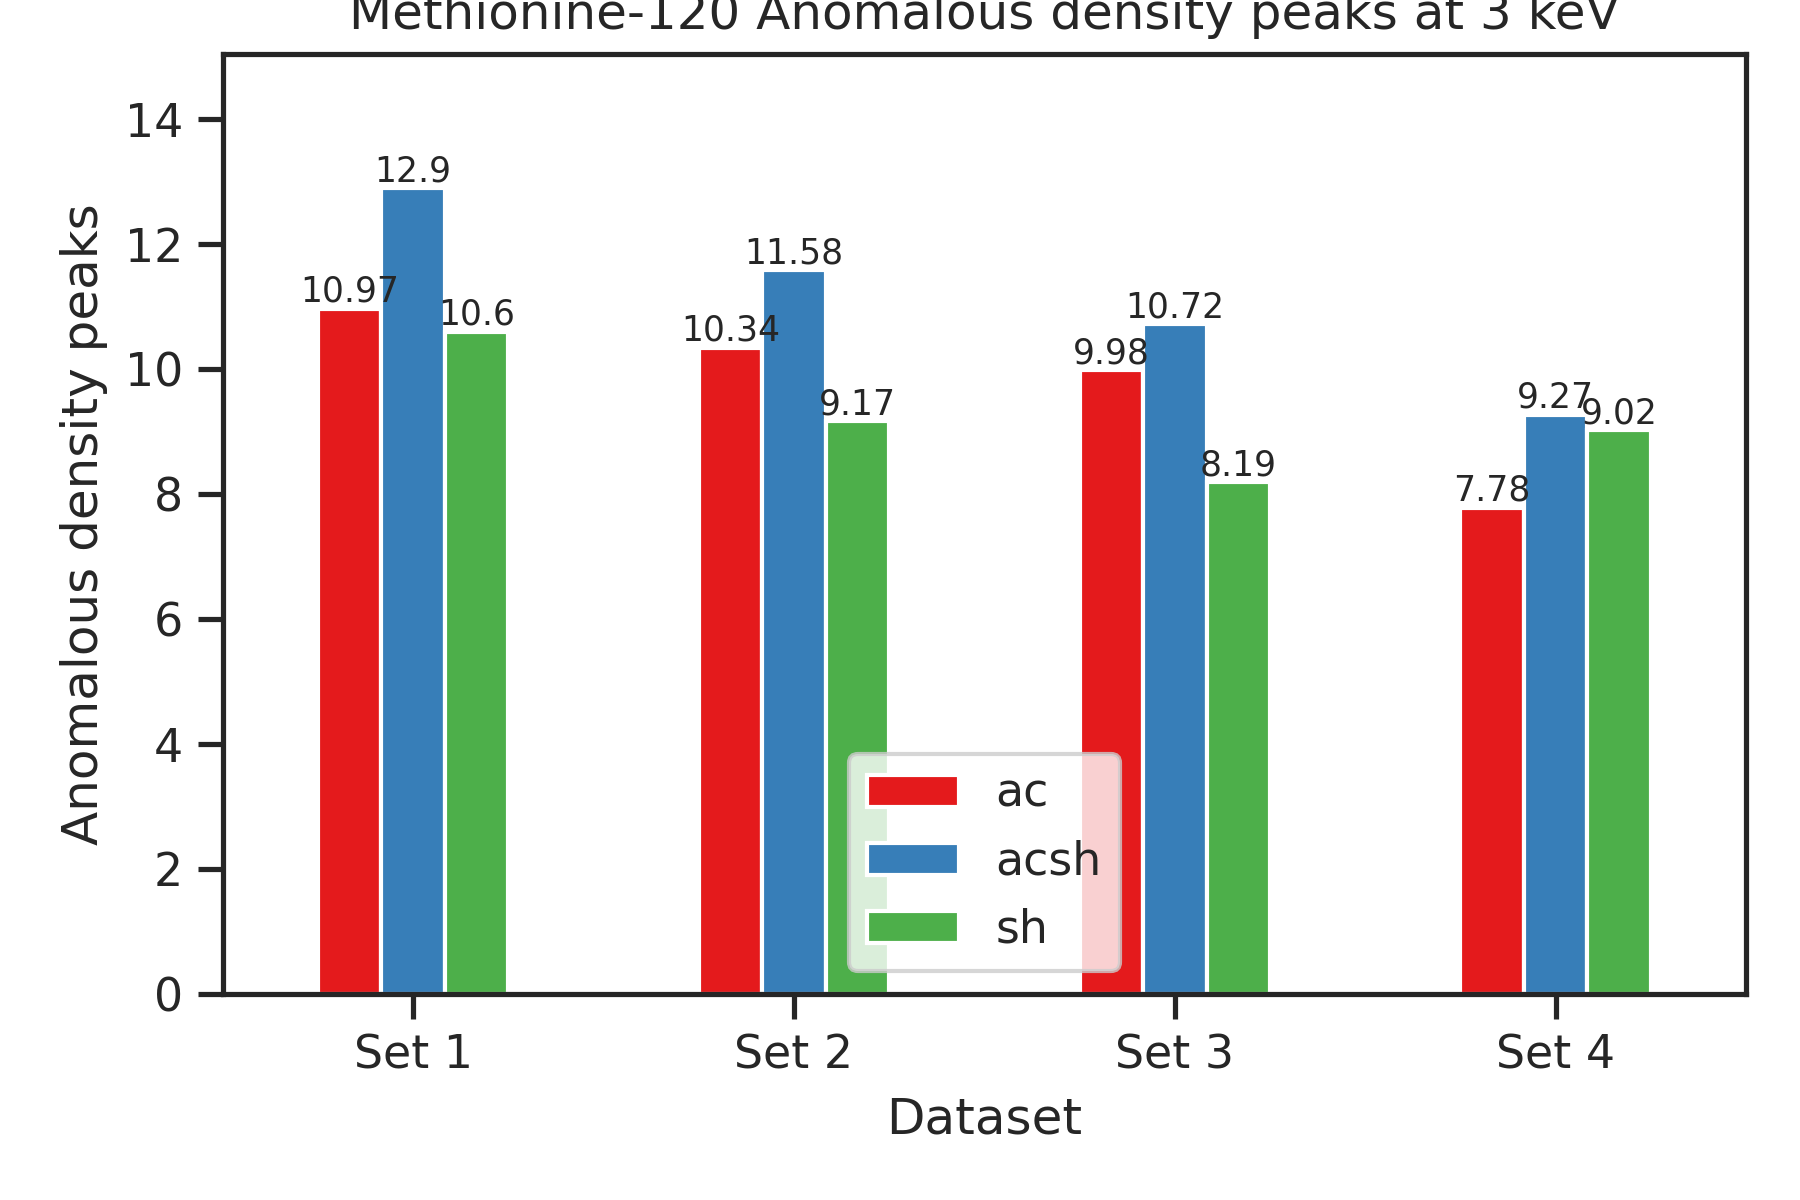
\includegraphics[width = 0.5\textwidth]{plots/exp1/tlys_2_P6122/peaks/3p0_m120_2Dbar.png} & 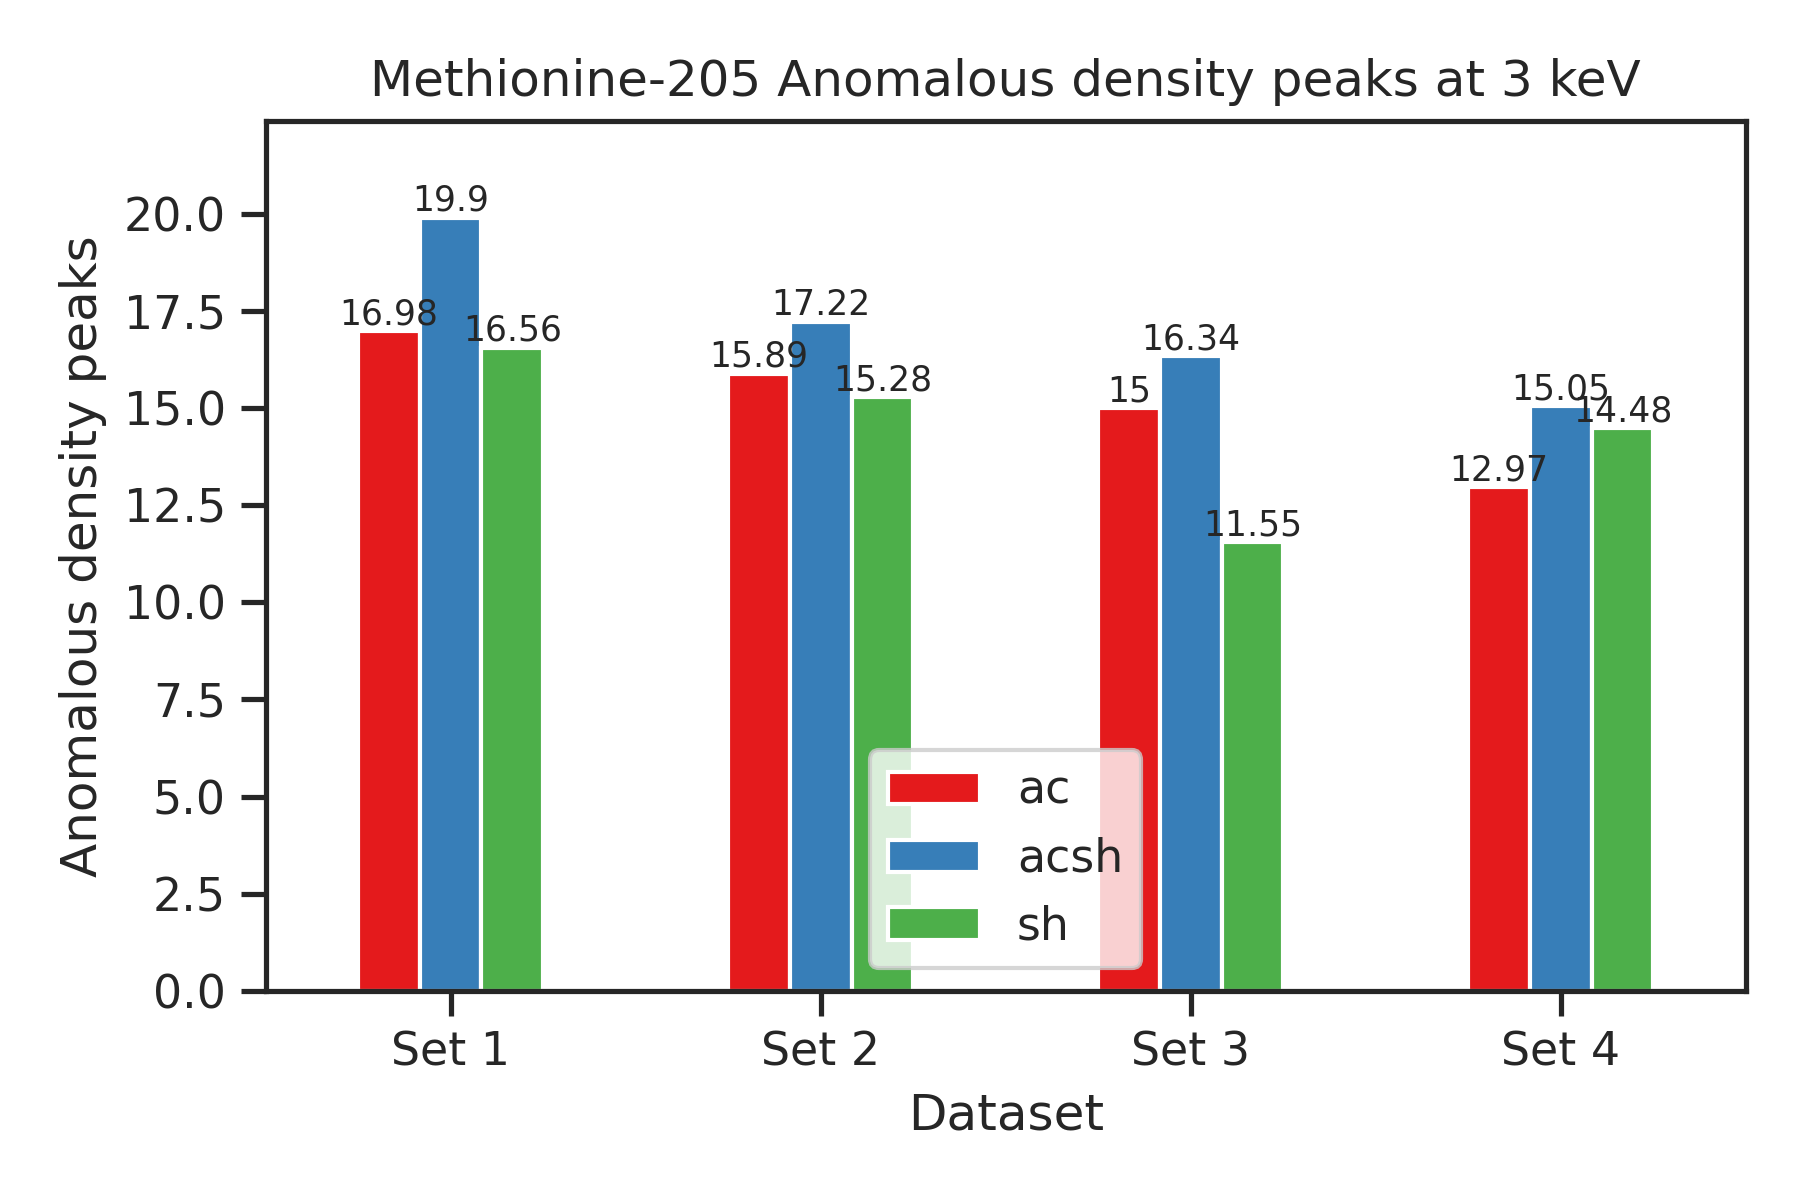
\includegraphics[width = 0.5\textwidth]{plots/exp1/tlys_2_P6122/peaks/3p0_m205_2Dbar.png}
    \end{tabular}
    \caption{Thermolysin 2: Anomalous density peaks of methionine groups at 3.0 \unit{keV}.}
    \label{fig:tlys2_met_peaks_3p0}
\end{figure}

\begin{figure}
    \centering
    \begin{tabular}{cc}
        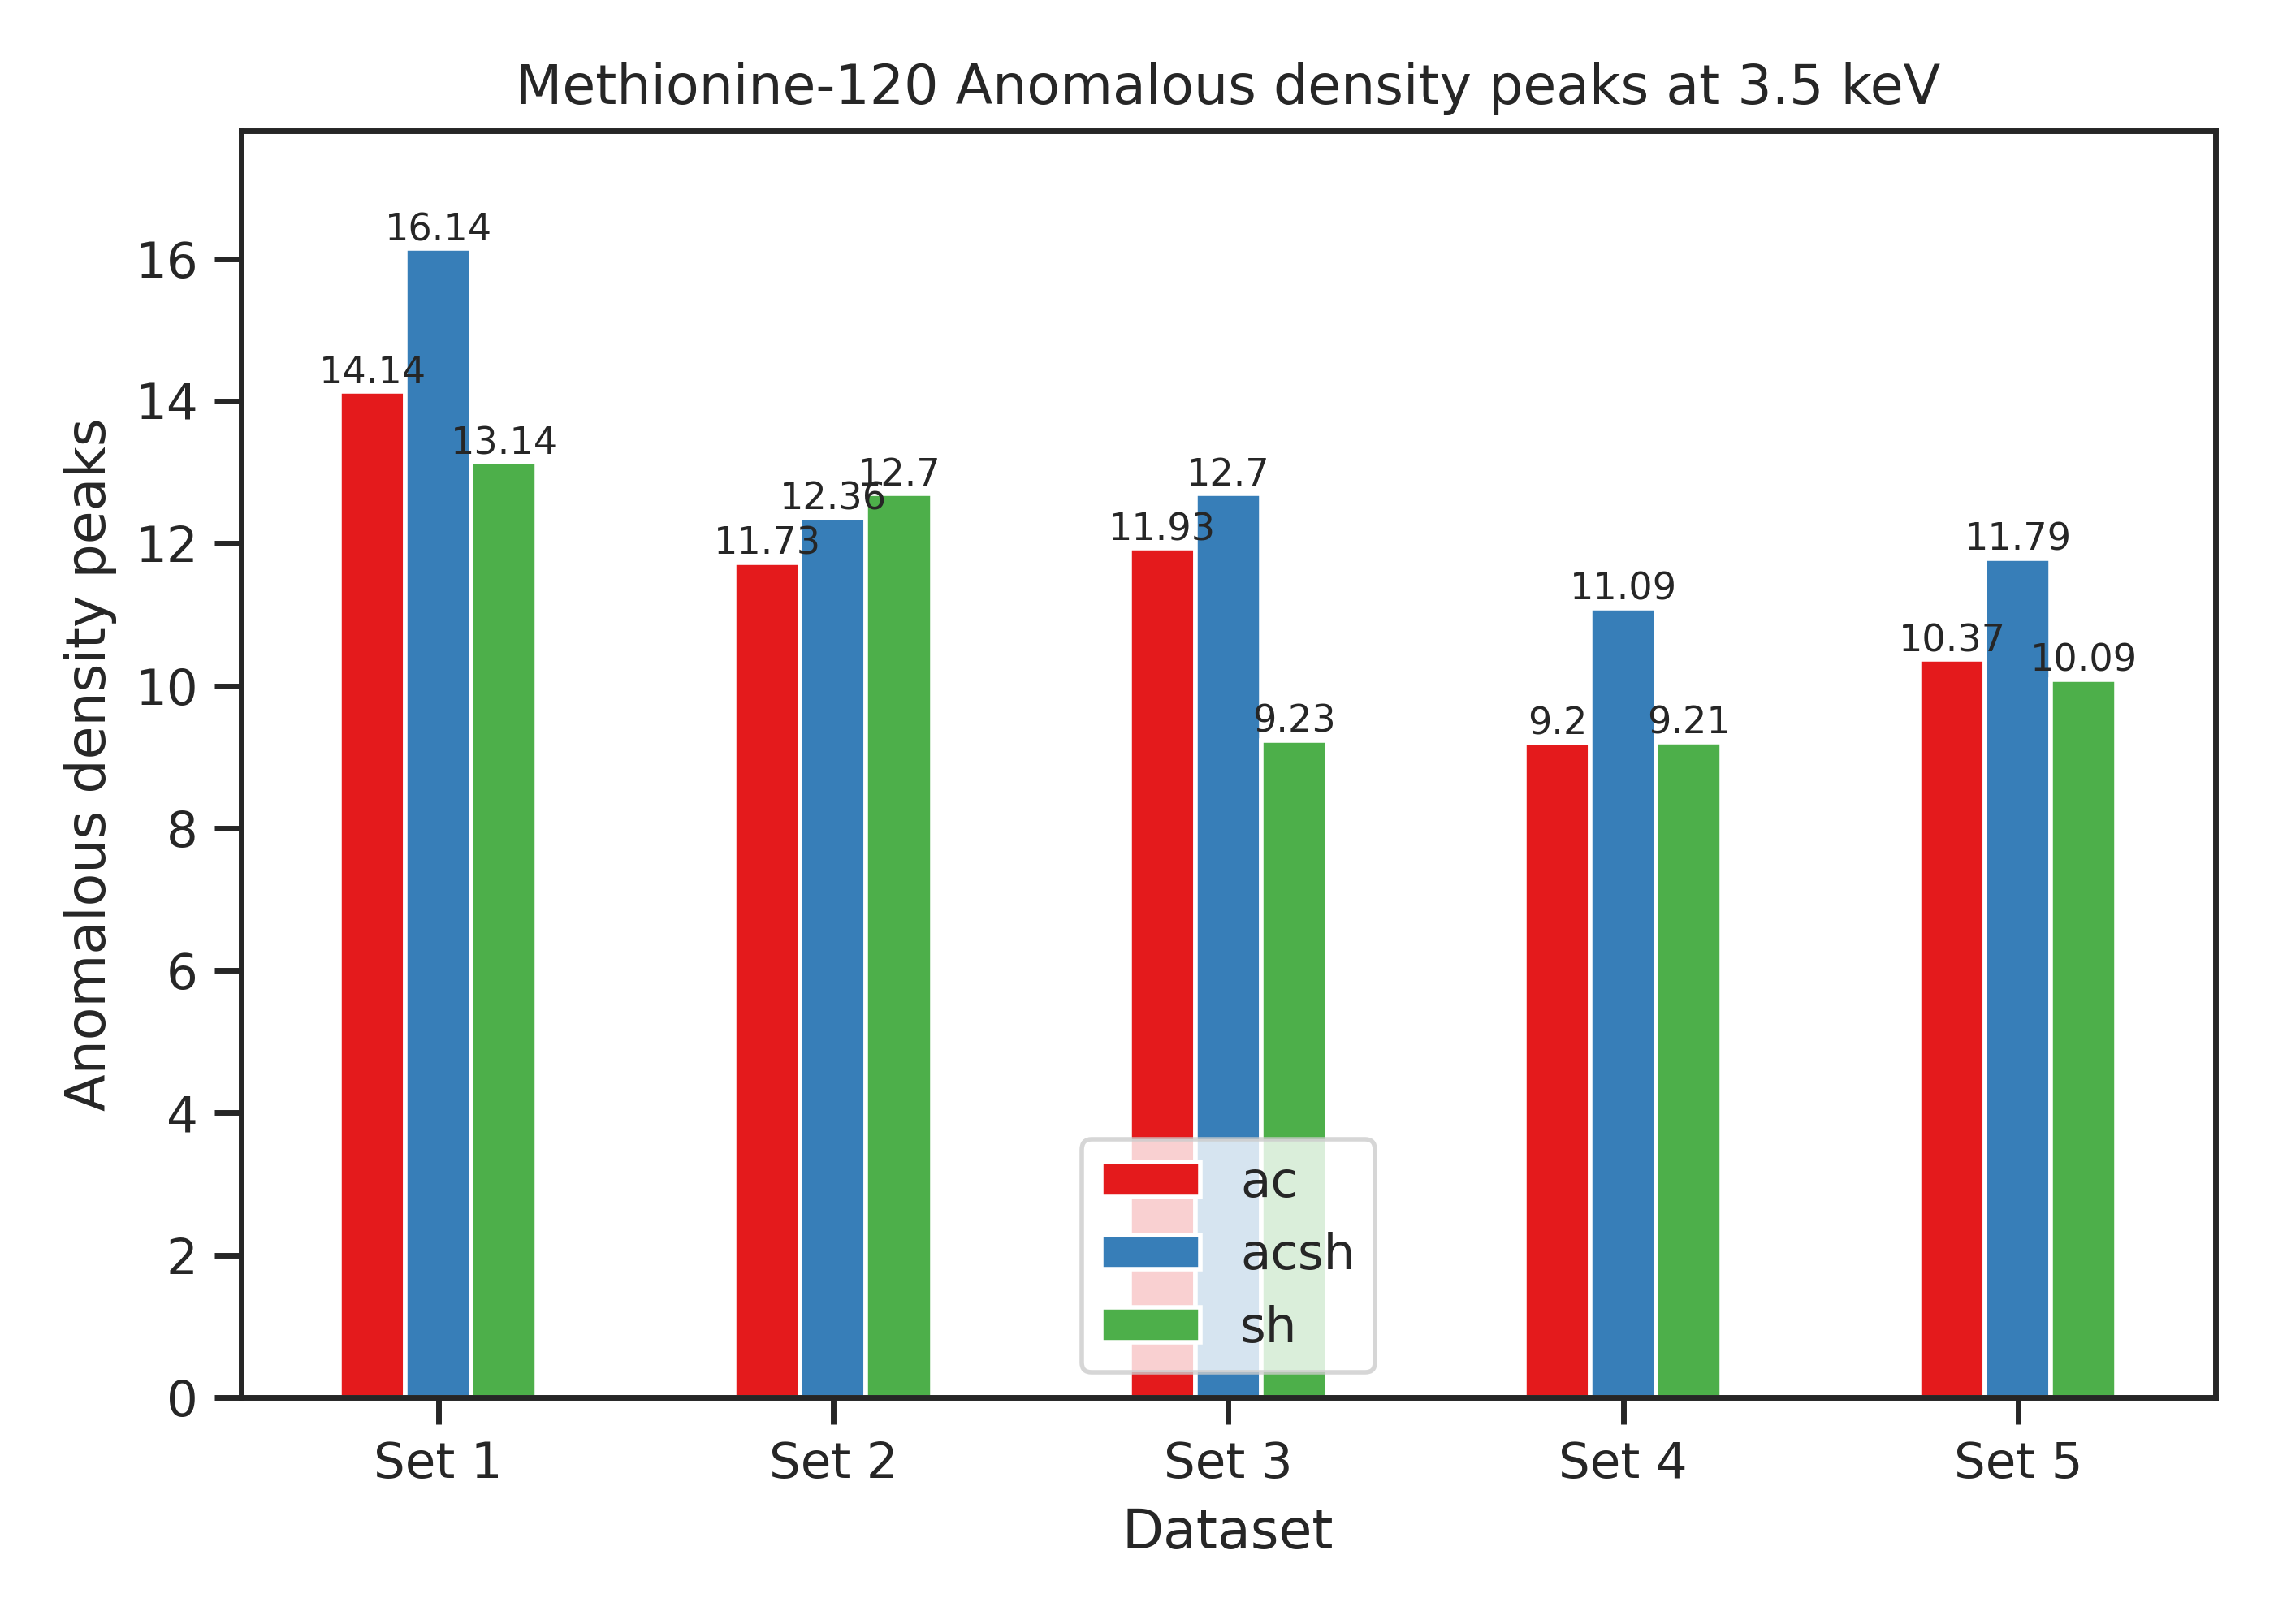
\includegraphics[width = 0.5\textwidth]{plots/exp1/tlys_2_P6122/peaks/3p5_m120_2Dbar.png} & 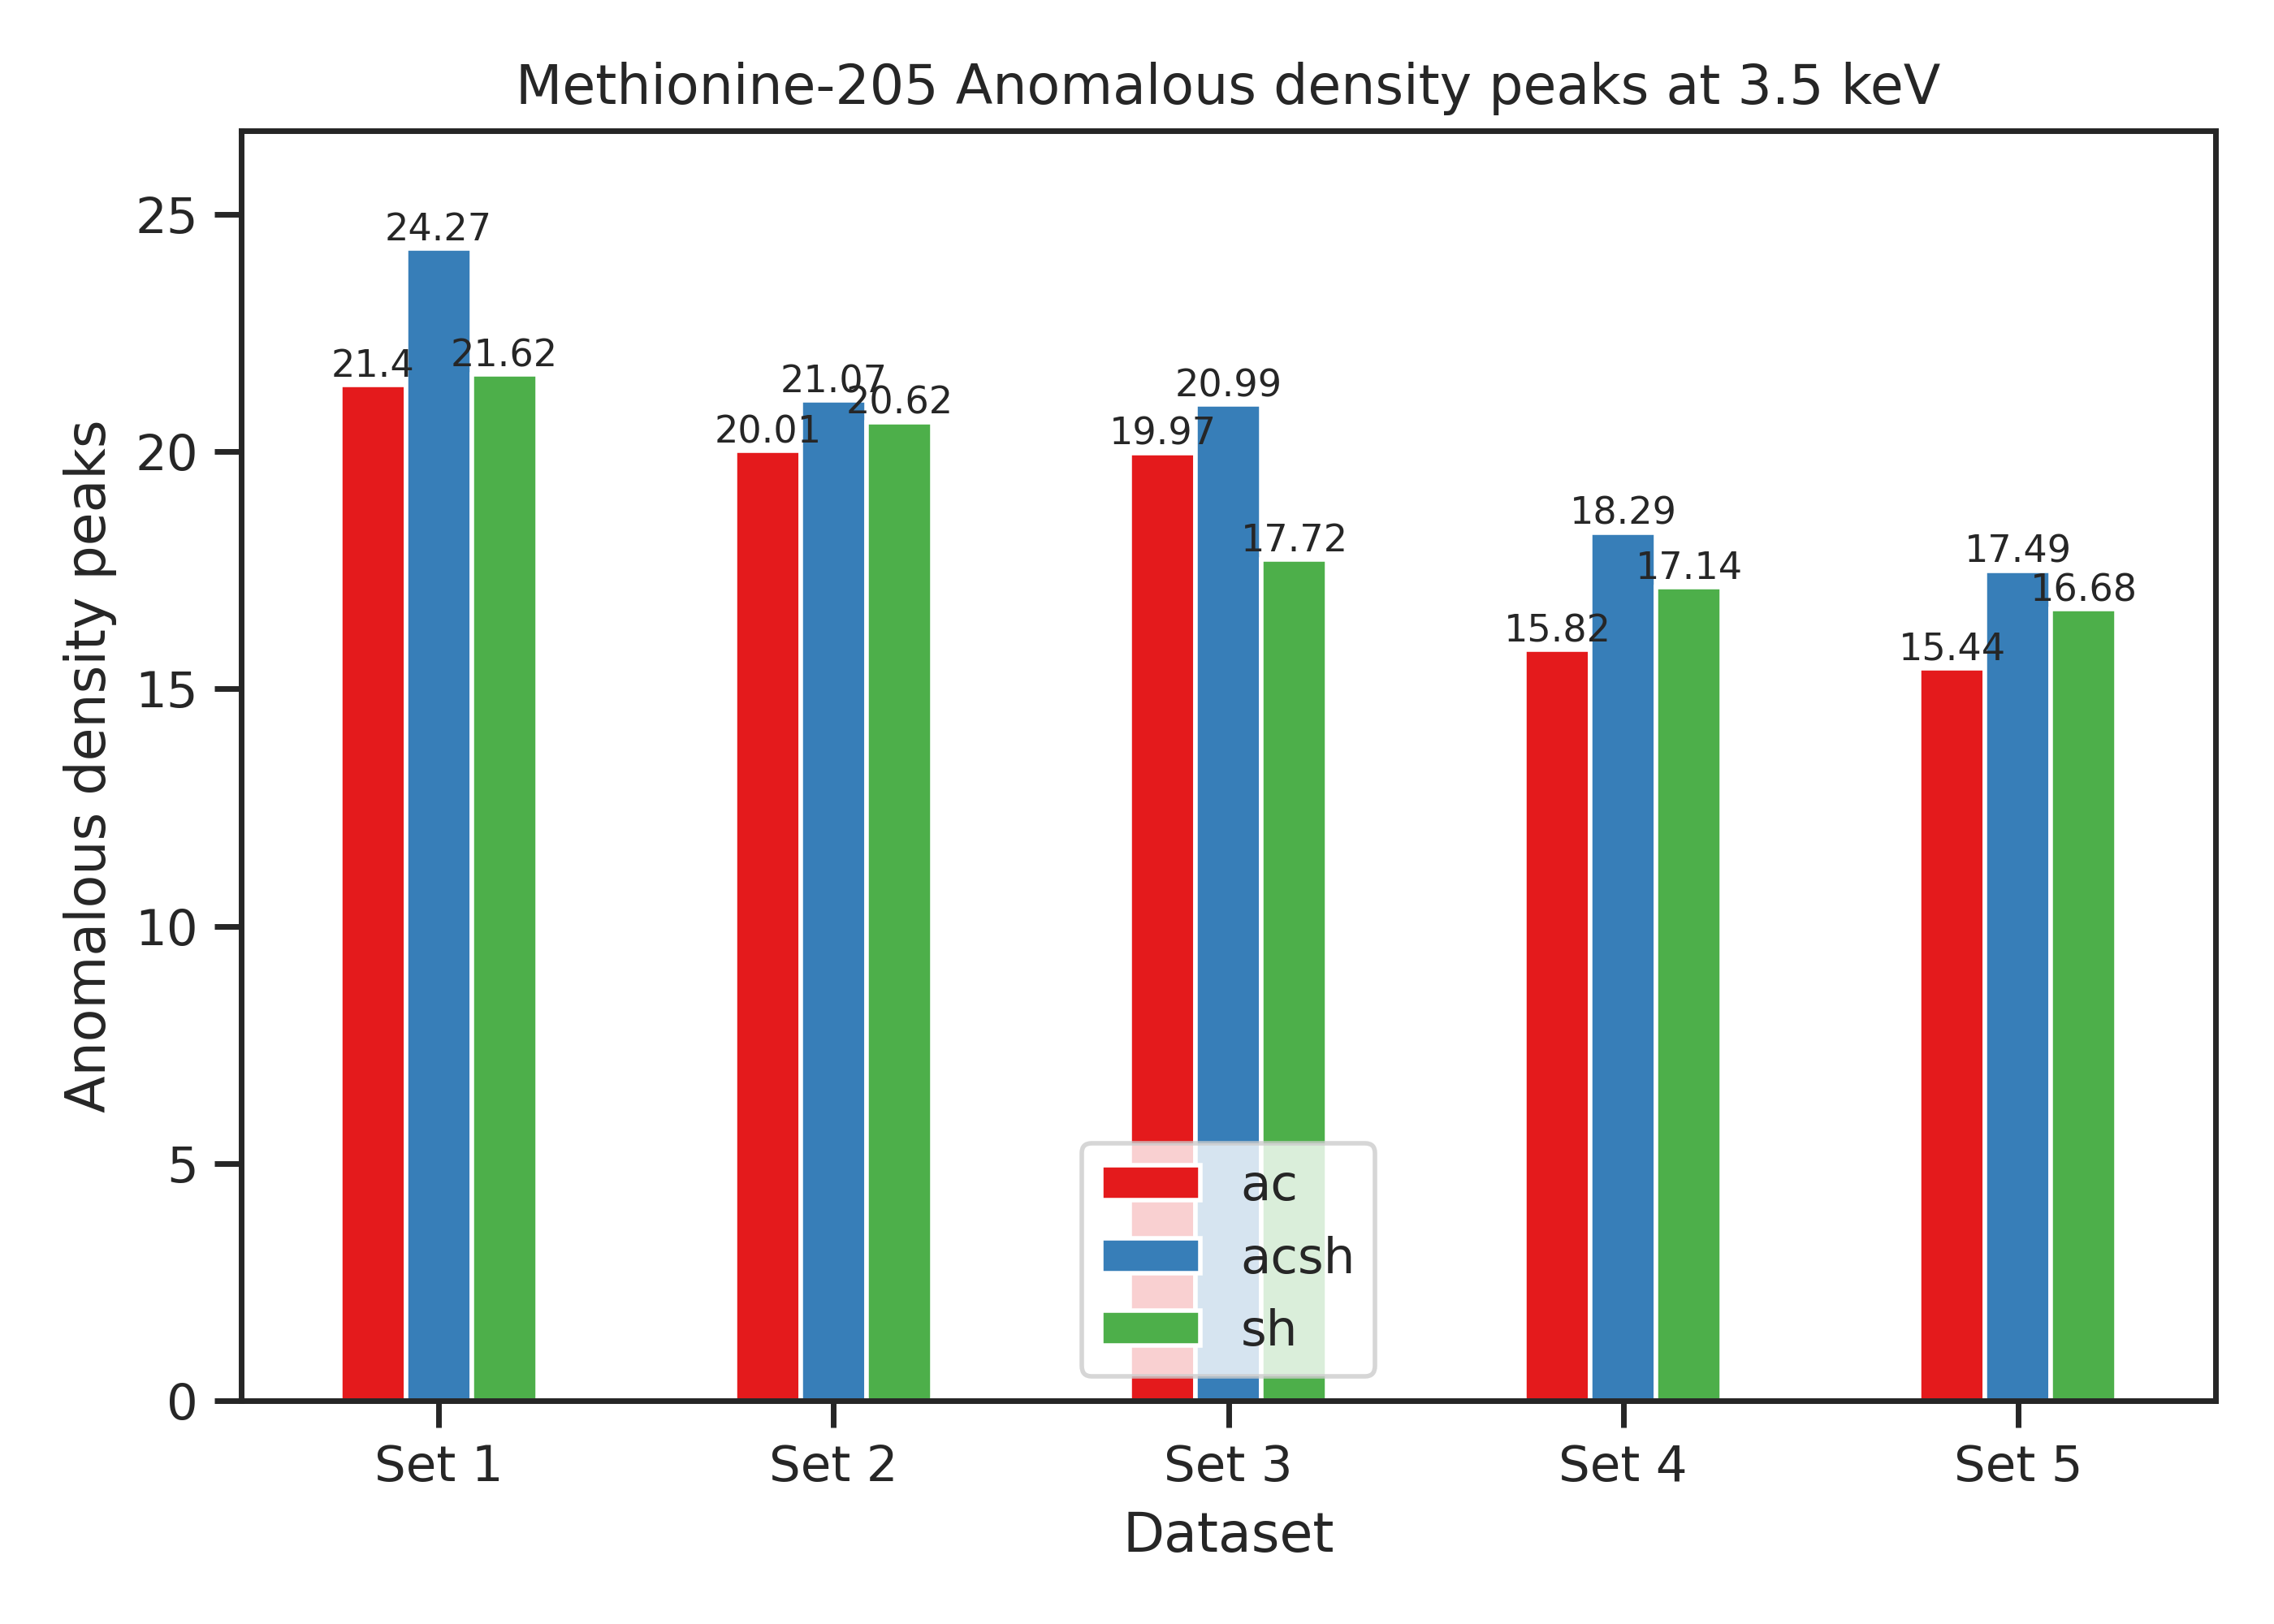
\includegraphics[width = 0.5\textwidth]{plots/exp1/tlys_2_P6122/peaks/3p5_m205_2Dbar.png}
    \end{tabular}
    \caption{Thermolysin 2: Anomalous density peaks of methionine groups at 3.5 \unit{keV}.}
    \label{fig:tlys2_met_peaks_3p5}
\end{figure}

\begin{figure}
    \centering
    \begin{tabular}{cc}
        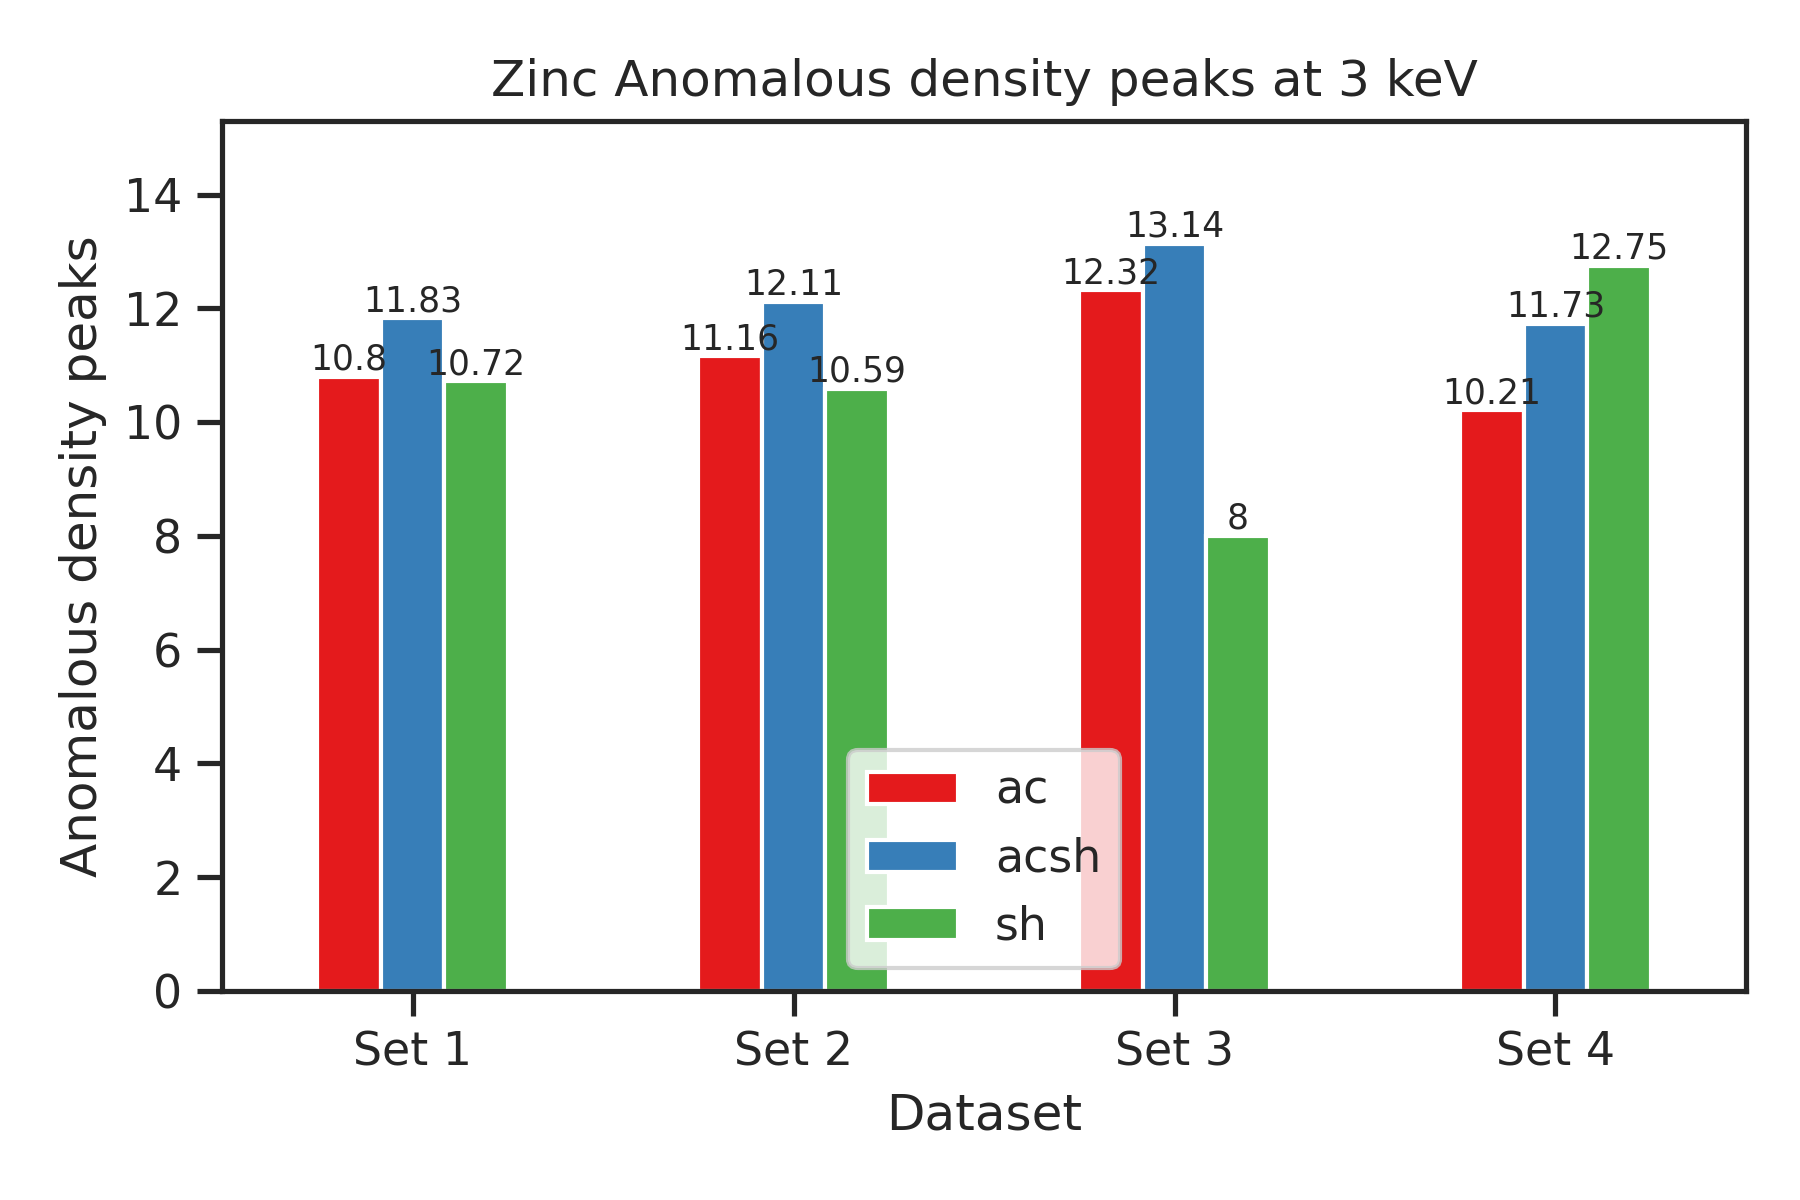
\includegraphics[width = 0.5\textwidth]{plots/exp1/tlys_2_P6122/peaks/3p0_zn_2Dbar.png} & 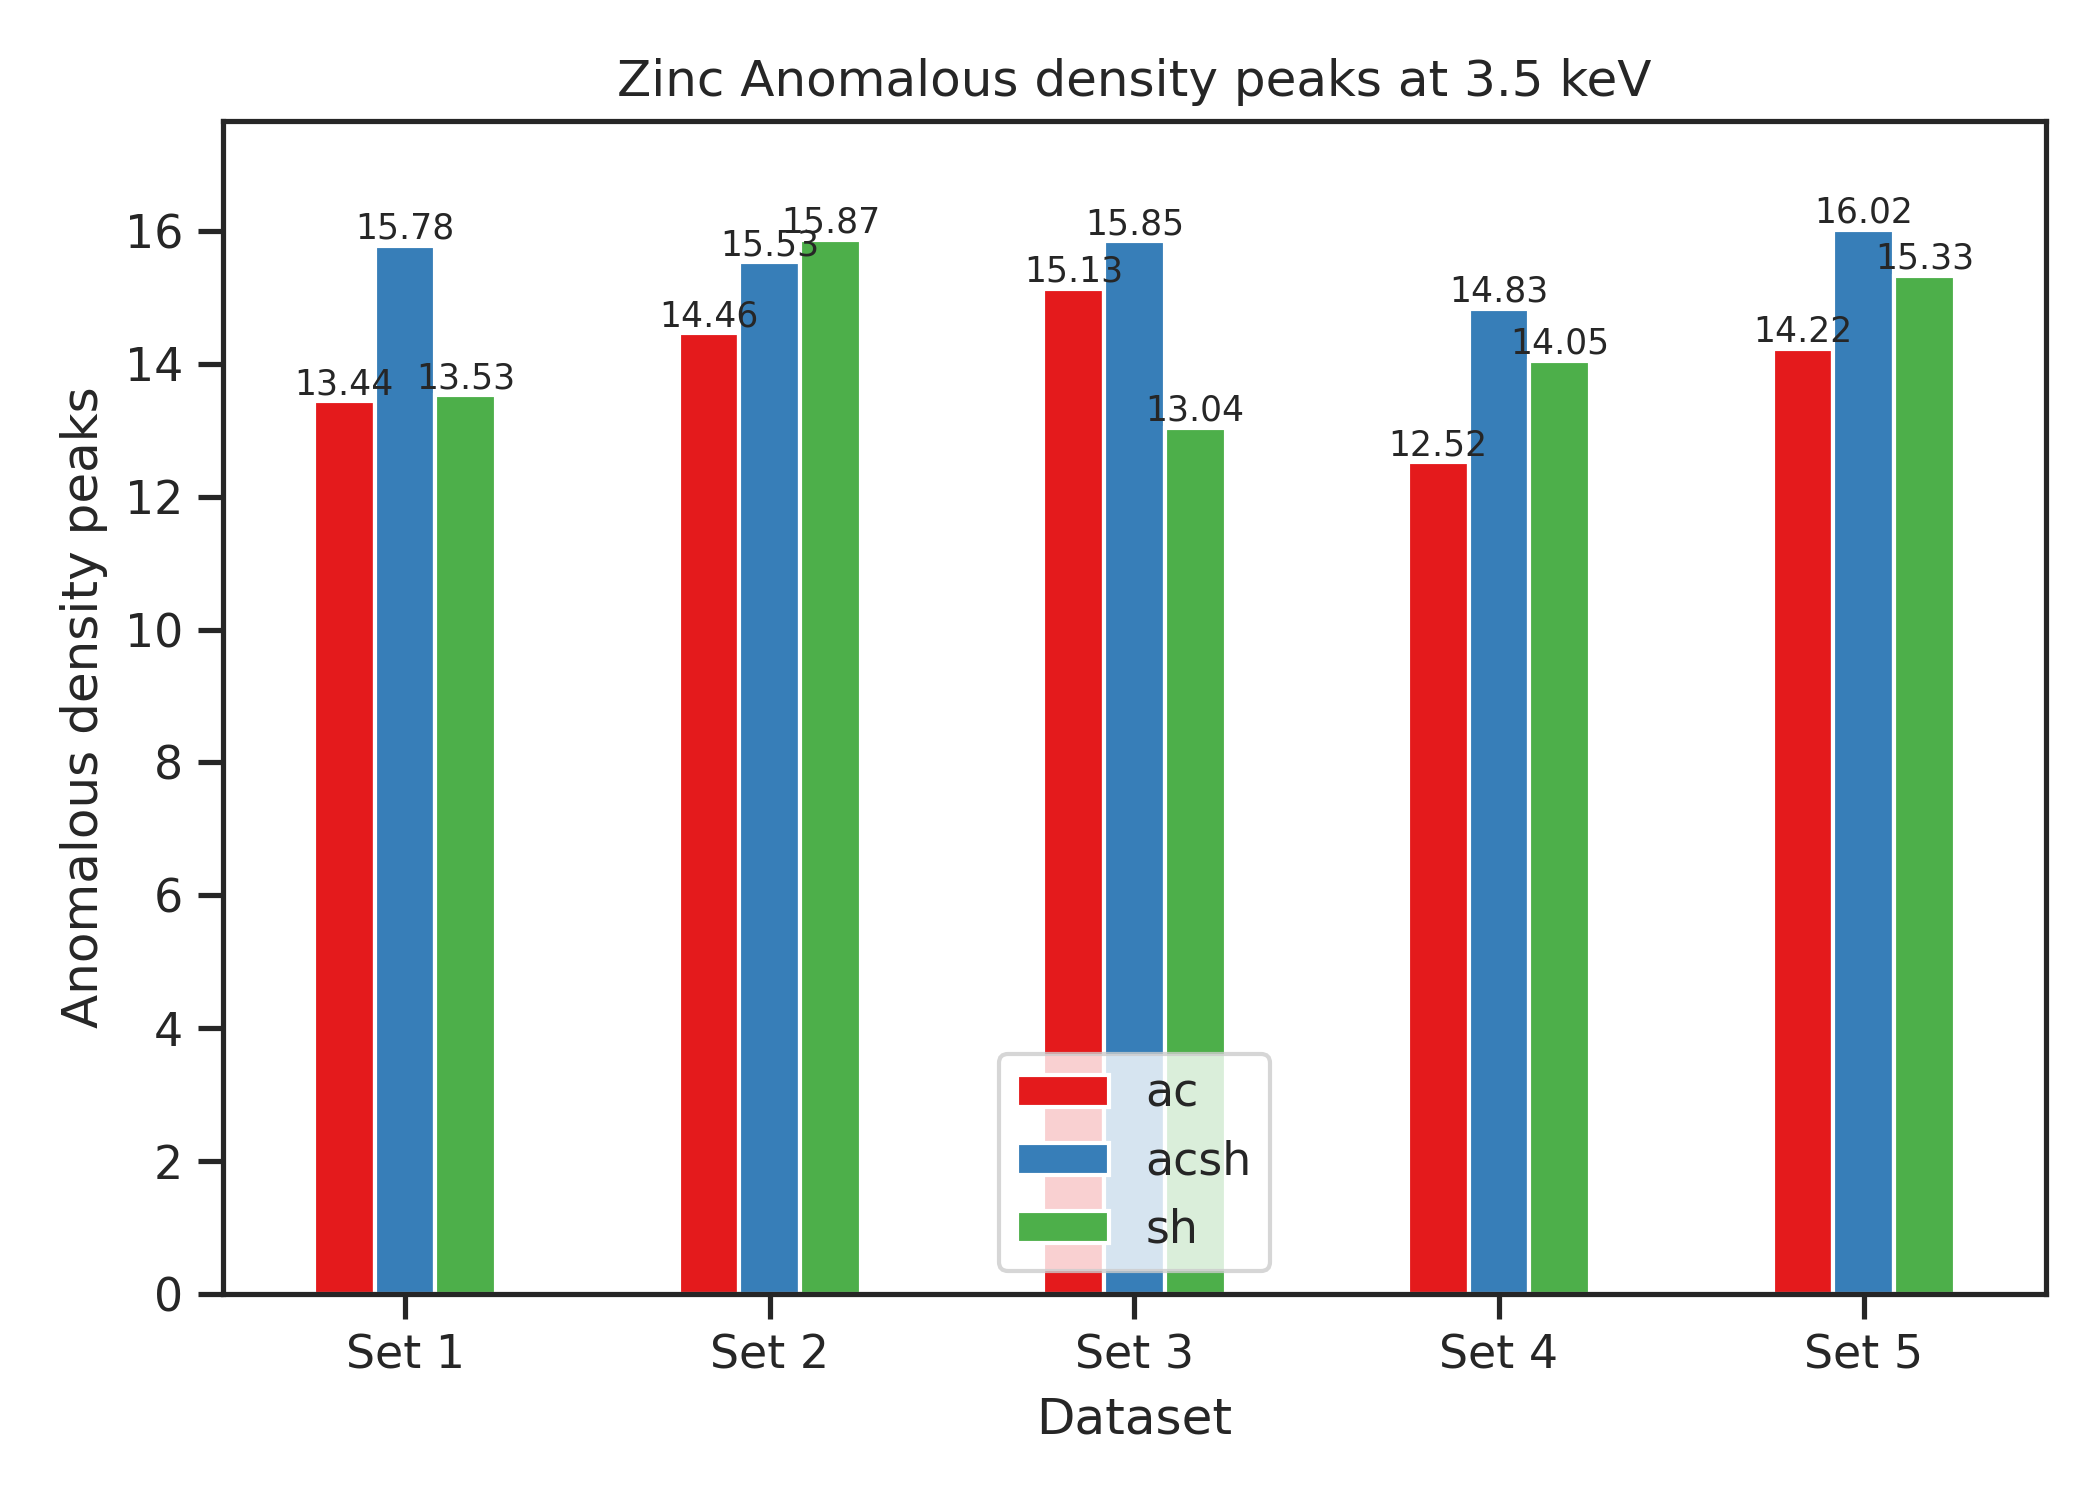
\includegraphics[width = 0.5\textwidth]{plots/exp1/tlys_2_P6122/peaks/3p5_zn_2Dbar.png}
    \end{tabular}
    \caption{Thermolysin 2: Anomalous density peaks of Zinc at 3.0 and 3.5 \unit{keV}.}
    \label{fig:tlys2_zn_peaks}
\end{figure}